% =====================================================================
%  Sentinel-RX: Security-Aware Agentic Recovery of Failing Systems
%  Technical Report -- Humain Hackathon, Challenge 1
%  Single self-contained LaTeX source (pdfLaTeX). No external .bib / .sty.
%  Figures: docs/technical_report/figures/*.png (copied from docs/figures by make report)
%  Every number in this document comes from results/*.json, results/summary.md,
%  docs/RESULTS.md, models/beacon_metrics.json or results/demo_live_trace.json.
% =====================================================================
\documentclass[11pt,a4paper]{article}

% ---------- encoding, fonts ------------------------------------------
\usepackage[T1]{fontenc}
\usepackage[utf8]{inputenc}
\usepackage{lmodern}
\usepackage{microtype}
\usepackage[table,dvipsnames]{xcolor}
\usepackage{amsmath,amssymb}
\usepackage{XCharter}
\usepackage[xcharter,vvarbb]{newtxmath}

% ---------- layout ---------------------------------------------------
\usepackage[a4paper,margin=2.5cm]{geometry}
\usepackage{graphicx}
\usepackage{adjustbox}
\graphicspath{{figures/}}
\usepackage{booktabs}
\usepackage{tabularx}
\usepackage{array}
\usepackage{siunitx}
\usepackage{algorithm}
\usepackage{algpseudocode}
\usepackage{enumitem}
\usepackage{caption}
\usepackage{subcaption}
\usepackage{float}
\usepackage[section]{placeins}
\usepackage{titlesec}
\usepackage{fancyhdr}
\usepackage[skins,breakable]{tcolorbox}
\usepackage{tikz}
\usetikzlibrary{arrows.meta,positioning,shapes.geometric,fit,backgrounds,calc,decorations.pathreplacing}
\usepackage{hyperref}
\usepackage{cleveref}

% ---------- palette --------------------------------------------------
\definecolor{accent}{HTML}{1F3A5F}     % navy
\definecolor{accent2}{HTML}{3C6E9F}    % lighter navy for rules
\definecolor{groupfill}{HTML}{E8F0FA}  % light blue group fill
\definecolor{outfill}{HTML}{FFF4CC}    % soft yellow outputs / evidence
\definecolor{detfill}{HTML}{E4F2EC}    % mint, detectors
\definecolor{llmfill}{HTML}{F1E8F7}    % lavender, LLM
\definecolor{safefill}{HTML}{FDEBD0}   % peach, safety
\definecolor{keyfill}{HTML}{F4F7FB}
\definecolor{limfill}{HTML}{FBF1F1}
\definecolor{decfill}{HTML}{F3F8F3}
\colorlet{attack}{red!75!black}
\definecolor{recovered}{HTML}{2E7D32}
\definecolor{muted}{HTML}{6B7280}

\hypersetup{colorlinks=true,linkcolor=accent,citecolor=accent2,urlcolor=accent2,
  pdftitle={Sentinel-RX: Security-Aware Agentic Recovery of Failing Systems},
  pdfauthor={Abdulrahman Alharbi}}

\sisetup{group-separator={\,},group-minimum-digits=4,detect-weight=true}
\captionsetup{font=small,labelfont={bf,color=accent},skip=6pt}
\setlist{nosep,leftmargin=*}

% ---------- headings -------------------------------------------------
\titleformat{\section}{\color{accent}\Large\bfseries}{\thesection}{0.8em}{}[{\color{accent2!50}\titlerule[0.6pt]}]
\titleformat{\subsection}{\color{accent}\large\bfseries}{\thesubsection}{0.8em}{}
\titleformat{\subsubsection}{\color{accent}\normalsize\bfseries}{\thesubsubsection}{0.8em}{}
\titlespacing*{\section}{0pt}{18pt}{8pt}
\titlespacing*{\subsection}{0pt}{12pt}{5pt}

% ---------- header / footer ------------------------------------------
\pagestyle{fancy}
\fancyhf{}
\fancyhead[L]{\small\color{muted}Sentinel-RX \textemdash\ Technical Report}
\fancyhead[R]{\small\color{muted}\thepage}
\renewcommand{\headrulewidth}{0.4pt}
\renewcommand{\headrule}{\color{accent2!50}\hrule width\headwidth height\headrulewidth}
\fancypagestyle{plain}{\fancyhf{}\renewcommand{\headrulewidth}{0pt}}

% ---------- boxes ----------------------------------------------------
\newtcolorbox{keyfinding}[1]{enhanced,breakable,colback=keyfill,colframe=accent,
  boxrule=0.6pt,arc=2pt,left=6pt,right=6pt,top=4pt,bottom=4pt,
  fonttitle=\bfseries\small,coltitle=white,colbacktitle=accent,title={Key finding \textemdash\ #1}}
\newtcolorbox{designdecision}[1]{enhanced,breakable,colback=decfill,colframe=recovered!70!black,
  boxrule=0.6pt,arc=2pt,left=6pt,right=6pt,top=4pt,bottom=4pt,
  fonttitle=\bfseries\small,coltitle=white,colbacktitle=recovered!70!black,title={Design decision \textemdash\ #1}}
\newtcolorbox{limitation}[1]{enhanced,breakable,colback=limfill,colframe=attack,
  boxrule=0.6pt,arc=2pt,left=6pt,right=6pt,top=4pt,bottom=4pt,
  fonttitle=\bfseries\small,coltitle=white,colbacktitle=attack,title={Limitation \textemdash\ #1}}
\newtcolorbox{summarybox}{enhanced,colback=groupfill,colframe=accent,boxrule=0.8pt,arc=3pt,
  left=8pt,right=8pt,top=6pt,bottom=6pt}

% ---------- tikz visual language -------------------------------------
\tikzset{
  box/.style={draw=accent,fill=white,rounded corners=3pt,align=center,font=\footnotesize,
              minimum height=7mm,inner sep=4pt,line width=0.6pt},
  service/.style={box,fill=groupfill,minimum width=17mm},
  detector/.style={box,fill=detfill},
  llm/.style={box,fill=llmfill},
  safety/.style={box,fill=safefill},
  output/.style={box,fill=outfill},
  good/.style={box,fill=recovered!12,draw=recovered!70!black},
  bad/.style={box,fill=attack!8,draw=attack},
  flow/.style={-{Stealth[length=2.2mm]},line width=0.7pt,draw=accent!85!black},
  beacon/.style={-{Stealth[length=2.2mm]},line width=0.9pt,draw=attack,dashed},
  lbl/.style={font=\tiny,text=muted,fill=white,inner sep=1.5pt,align=center},
  group/.style={draw=accent!55,dashed,rounded corners=6pt,fill=groupfill!45,inner sep=9pt},
  grouplbl/.style={font=\scriptsize\bfseries,text=accent,anchor=south west,inner sep=2pt},
  decision/.style={diamond,aspect=2.4,draw=accent,fill=white,align=center,font=\footnotesize,
                   inner sep=1.5pt,line width=0.6pt},
  brace/.style={decorate,decoration={brace,amplitude=4pt},draw=accent2},
}

\newcommand{\code}[1]{\texttt{#1}}
\newcommand{\pct}[1]{#1\,\%}
\newcommand{\ci}[2]{{\footnotesize[#1,\,#2]}}

\begin{document}

% =====================================================================
%  TITLE PAGE
% =====================================================================
\begin{titlepage}
\thispagestyle{empty}
\vspace*{2.2cm}
\noindent{\color{accent}\rule{\textwidth}{1.2pt}}\\[1.2em]
{\color{accent}\Huge\bfseries Sentinel-RX}\\[0.4em]
{\color{accent}\LARGE\bfseries Security-Aware Agentic Recovery of Failing Systems}\\[1.0em]
{\large Technical Report \textemdash\ Humain Hackathon, Challenge~1: Agentic Recovery of a Failing System}\\[0.6em]
{\color{accent}\rule{\textwidth}{1.2pt}}

\vspace{2.0cm}
{\large\bfseries Abdulrahman Alharbi}\\[0.3em]
{\large 30 October 2026}

\vspace{2.2cm}
\begin{summarybox}
\small\textbf{Summary.}
Sentinel-RX is an agent that identifies, diagnoses, recovers and \emph{verifies} the recovery of a
failing enterprise system in which several faults are active at once and a security compromise may
hide inside an operational incident. Four cheap deterministic detectors (robust metric z-scores,
log-template signatures, a dependency-aware root-cause ranker and a RandomForest beacon detector)
compress thousands of telemetry records into a short ranked evidence list; a local 7B model
(\code{qwen2.5:7b} via Ollama) reasons over it inside a MAPE-K loop with a step budget; a safety layer
enforces an action allowlist, contain-before-restart for compromised hosts and transactional rollback;
and a verification gate permits a ``recovered'' claim only when post-action telemetry matches the
pre-incident baseline and no beacon attempt remains. On 20 held-out incidents never used during
development (3 seeds, $n=60$) the agent recovers \pct{100} of systems with \pct{0} false claims and
zero harmful actions, against \pct{45} for a rule-based runbook and \pct{30} for a single-shot LLM
that falsely claims recovery \pct{70} of the time. The benchmark, the simulator, a live five-process
environment, a replay cache that makes every number reproducible without an LLM, and 109 tests ship
with the code. Everything ran on one laptop with no cloud and no Docker.
\end{summarybox}
\vfill
{\small\color{muted}Repository: \code{github.com/AbdulAlharbi/sentinel-rx} (reproduction commands in Appendix~\ref{app:repro}).
Literature review: \code{docs/literature\_review.pdf}.}
\end{titlepage}

% =====================================================================
%  EXECUTIVE SUMMARY
% =====================================================================
\pagestyle{plain}
\section*{Executive summary}
\addcontentsline{toc}{section}{Executive summary}

\textbf{Problem.} Automated incident recovery is evaluated almost exclusively on single, accidental
faults. Real incidents involve several interacting faults, symptoms that propagate along service
dependencies, and sometimes a compromise that looks like a performance problem. An agent that
restarts a compromised host destroys evidence and lets the implant re-establish; an agent that
declares ``recovered'' without checking is worse than no agent at all.

\textbf{What was built.} A complete, locally reproducible system and benchmark:
\begin{itemize}
  \item a deterministic simulator of a five-service enterprise with dependency propagation, nine
        known fault types plus one held-out unseen type, and hidden ground truth;
  \item a live environment of five real local processes with real memory growth, a real dead
        process, a real connection-pool hold and real periodic HTTP beacons to a local sinkhole;
  \item the agent: detectors $\rightarrow$ LLM hypotheses and targeted checks $\rightarrow$ ordered
        plan $\rightarrow$ safety layer $\rightarrow$ verification gate, two LLM calls per iteration;
  \item a benchmark with dev/held-out split enforcement, perturbations, six baselines and sanity
        floors, four ablations, bootstrap confidence intervals, and a mid-development scorer audit.
\end{itemize}

\textbf{Headline result (held-out, \code{qwen2.5:7b}, 20 scenarios $\times$ 3 seeds).}
\begin{center}\footnotesize
\setlength{\tabcolsep}{5pt}
\adjustbox{max width=\textwidth}{%
\begin{tabular}{lrrrrr}
\toprule
configuration & top-1 root cause & recovered & false ``recovered'' & harmful / run & LLM tokens / run \\
\midrule
\rowcolor{groupfill}\textbf{Sentinel-RX agent} & \pct{92} & \pct{100} & \pct{0} & 0.00 & \num{6103} \\
runbook (rules, no LLM) & \pct{87} & \pct{45} & \pct{5} & 0.00 & 0 \\
single-shot LLM & \pct{63} & \pct{30} & \pct{70} & 0.27 & \num{2421} \\
LLM only (no detectors, $n=20$) & \pct{35} & \pct{35} & \pct{15} & 0.55 & \num{35018} \\
do-nothing / random floors & \pct{0} & \pct{0} & \pct{0} / \pct{10} & 0.00 / 3.45 & 0 \\
\bottomrule
\end{tabular}}
\end{center}

\textbf{Why it works.} Ablations show each component protects a different metric: removing the
verification gate raises false claims from \pct{0} to \pct{80}; removing the loop drops recovery
to \pct{20}; removing the beacon detector drops recovery to \pct{50} and raises false claims to
\pct{35}; removing the safety layer keeps recovery at \pct{100} but introduces 0.60 harmful actions
per run. Under noisy logs, missing metrics, renamed services, timestamp jitter and an unseen fault
type, recovery stays at \pct{95}--\pct{100} (the unseen type is recovered, not identified). A 1.5B model recovers only \pct{50} but still makes
\pct{0} false claims and zero harmful actions, because those guarantees live in the detectors,
the safety layer and the verifier rather than in the model.

\textbf{Honesty.} A scorer audit during development found that early versions were \emph{not}
harmless (0.27 and 0.23 containment actions per run on uncompromised hosts hidden by the old
scorer) and that the observable health formula was too lenient; both were fixed, all earlier runs
were re-scored, and the do-nothing and random baselines remain in the benchmark as permanent
sanity floors. Several evaluation arms use one seed because of the laptop time budget; their
deltas are directional.

\clearpage
\tableofcontents
\clearpage
\pagestyle{fancy}

% =====================================================================
\section{Introduction}
% =====================================================================

Incident response is the most expensive and least automated stage of operating software. An
on-call engineer must notice that something is wrong, localise it in a dependency graph where every
downstream fault produces upstream symptoms, decide what to do, do it without making things worse,
and confirm that the system is actually healthy again. The post-2023 literature has moved from
``can a model rank likely root causes?'' to ``can an agent own the incident end to
end?''~\cite{aiopslab,itbench,stratus}, yet reported success rates on realistic benchmarks remain
around \pct{11}~\cite{openrca,itbench}, and evaluations almost never address three things that make
real incidents hard.

\paragraph{Concurrent faults.} With one fault per scenario, the deepest anomalous service is the
answer. With two or three, the symptom pattern is a superposition: a memory leak on \code{api} and a
connection-pool exhaustion on \code{db} both show up as errors on \code{api} and \code{gateway}.
Classical root-cause analysis assumes a single cause; a model that fixes one fault and sees the
symptom persist must decide whether its fix was wrong or merely incomplete.

\paragraph{Hidden security incidents.} A command-and-control (C2) beacon adds a few percent of CPU
and a handful of small periodic outbound flows hidden among health checks and update polls. If an
ops agent treats the host like any slow service and restarts it, it destroys forensic evidence and
the implant re-establishes. The correct order is \emph{contain, then eradicate}, and no AIOps
benchmark we reviewed tests that~\cite{itbench,aiopslab}.

\paragraph{Verification.} An agent that declares success is believed. A false ``recovered'' claim
closes the incident with the fault still active, which is strictly worse than escalating. Mitigation
success is measured in the literature; false recovery as a distinct error class almost never is.

\subsection{Contributions}
\begin{enumerate}
  \item \textbf{A security-aware hybrid agent} (\cref{sec:overview,sec:impl,sec:algo}): deterministic
        detectors feed a local 7B model inside a budgeted MAPE-K loop; a safety layer enforces an
        allowlist, evidence-gated containment, contain-before-restart ordering and transactional
        rollback; a verification gate compares post-action telemetry with the remembered healthy
        baseline before any recovery claim.
  \item \textbf{A reproducible benchmark} (\cref{sec:eval}): a deterministic simulator with dependency
        propagation and hidden ground truth, 30 development and 20 held-out multi-fault scenarios with
        disjoint fault combinations, five perturbations including an unseen fault type, six baselines
        (two of them sanity floors), four ablations, exact metric definitions and bootstrap CIs. A
        content-addressed LLM cache makes every reported number replayable with no model installed.
  \item \textbf{Evidence on all five literature gaps} (\cref{sec:results}): the agent reaches
        \pct{100} recovery, \pct{0} false claims and zero harmful actions on held-out incidents at
        \num{6103} tokens per incident, while the raw-telemetry variant of the same loop needs
        \num{35018} tokens to recover \pct{35}.
  \item \textbf{A live environment} (\cref{sec:live}): the same agent, byte-identical, recovers a
        real three-fault incident on five real processes, containing the beaconing host before
        restarting it.
  \item \textbf{An audited scorer} (\cref{sec:audit}): the recovery metric was challenged
        mid-development, found lenient in two places, fixed, and all earlier runs re-scored.
\end{enumerate}

% =====================================================================
\section{State of the Field}
\label{sec:sota}
% =====================================================================

The conceptual skeleton of every agentic design is still Kephart and Chess's autonomic computing
vision~\cite{kephart}: a Monitor--Analyze--Plan--Execute loop over shared knowledge (MAPE-K). Chaos
engineering~\cite{chaos} supplies the evaluation method: inject real faults and measure deviation
from a hypothesised steady state. Surveys of pre-LLM AIOps~\cite{notaro} consistently find
remediation the least mature stage.

\paragraph{Hybrid evidence collection in production.} RCACopilot~\cite{rcacopilot} separates
deterministic, incident-specific handlers that gather multi-source diagnostic data from an LLM that
predicts the root-cause category with an explanation (Micro-F1 up to 0.766 on a year of Microsoft
incidents). RCAgent~\cite{rcagent} moves to a ReAct-style~\cite{react} controller with
information-gathering tools and, importantly for this project, an \emph{internally deployed} model
plus structured-output repair that sharply reduces invalid actions. Both establish the principle
Sentinel-RX follows: deterministic tooling gathers evidence, the LLM reasons over it.

\paragraph{Interactive benchmarks.} AIOpsLab~\cite{aiopslab,aiopslab-vision} deploys fault-injected
microservices behind an agent--cloud interface with 48 problems across detection, localisation, RCA
and mitigation. ITBench~\cite{itbench} spans SRE, CISO and FinOps scenarios; state-of-the-art agents
resolved about \pct{11} of SRE and \pct{25} of CISO scenarios. OpenRCA~\cite{openrca} provides 335
real failures with 68\,GB of telemetry; the best agent identifies the full root cause in about
\pct{11} of cases and often reaches correct answers through flawed reasoning. RCAEval~\cite{rcaeval}
standardises AC@$k$ over 735 cases and 11 fault types. All of them inject one fault per scenario.

\paragraph{Safety of autonomous remediation.} STRATUS~\cite{stratus} organises specialised
detection, diagnosis and mitigation agents in a state machine and formalises \emph{transactional
no-regression}: a mitigation that does not improve the system is rolled back. ToolEmu~\cite{toolemu}
shows that even the safest tool-using agents exhibit risky behaviour in \pct{23.9} of test cases.
Neither addresses whether an action is \emph{appropriate} to the nature of the incident, for example
restarting a compromised container.

\paragraph{C2 beaconing.} BAYWATCH~\cite{baywatch} detects stealthy beaconing in enterprise proxy
logs via signal processing and emphasises that legitimate software also beacons, making false
positives the central challenge. CTU-13~\cite{ctu13} remains the standard labelled botnet dataset.
The author's prior work~\cite{alharbi-thesis} showed that periodicity features computed from flow
timestamps alone (inter-arrival regularity, spectral concentration, autocorrelation, sub-window
stability) rank suspicious communication on encrypted traffic (AP 0.852 vs.\ 0.046 for a heuristic
on CTU-13 with synthetic beacon injection). These features are cheap and payload-free, which makes
them usable as a deterministic detector inside an operations agent.

\paragraph{Gaps.} The review (\code{docs/literature\_review.pdf}) ends with five gaps that define
this project's research questions:
\begin{description}[style=nextline,font=\bfseries\color{accent}]
  \item[G1 Concurrent and confounded faults.] Evaluations inject one fault; classical RCA assumes one cause.
  \item[G2 Security-blind operations.] No AIOps benchmark checks whether an agent recognises a compromise inside an operational fault, or whether its remediation is appropriate when it does.
  \item[G3 Verification of recovery.] Agents falsely declaring recovery is rarely reported as a distinct error class.
  \item[G4 Cost of the agent.] Tokens, latency and compute per incident are seldom reported; most evaluations use large proprietary models.
  \item[G5 Robustness and generalisation.] Telemetry degradation and held-out fault combinations are rarely tested systematically.
\end{description}

% =====================================================================
\section{System Overview}
\label{sec:overview}
% =====================================================================

\Cref{fig:arch} shows the whole system. The agent never sees the simulator's fault list; it talks to
an environment only through the \code{Env} interface (status, metrics, logs, flows, actions). Raw
telemetry goes through four deterministic detectors that emit a short ranked evidence list. The LLM
turns evidence into ranked hypotheses and up to three targeted checks, then into an ordered plan.
The safety layer screens and reorders the plan, executes it transactionally, and the verification
gate decides whether the system is healthy by comparing post-action telemetry with the healthy
baseline remembered at the first observation. The C2 sinkhole stands in for the attacker's server:
in the simulator it is a destination address, in the live environment a real local HTTP process.

\begin{figure}[H]
\centering
\adjustbox{max width=\textwidth}{%
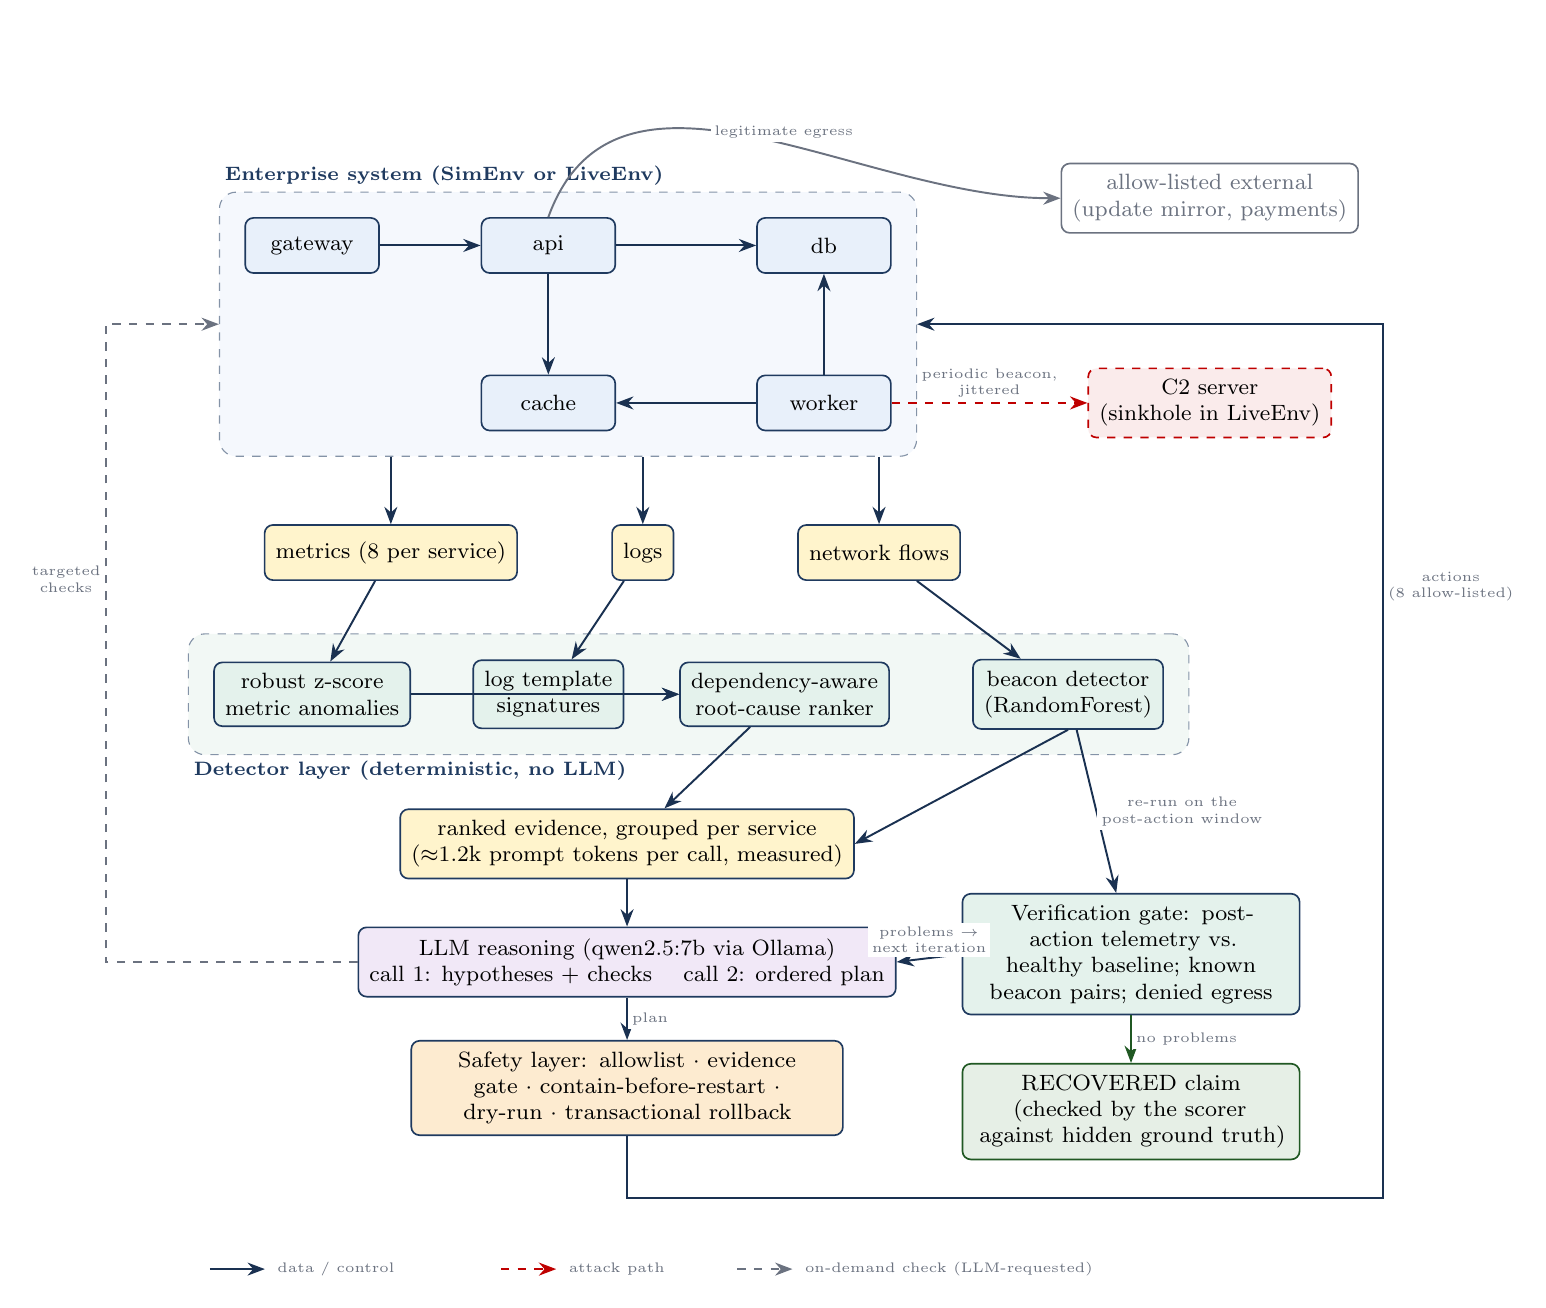
\begin{tikzpicture}
  % ---- enterprise system ----
  \node[service] (gw) at (0,2) {gateway};
  \node[service] (api) at (3,2) {api};
  \node[service] (db) at (6.5,2) {db};
  \node[service] (cache) at (3,0) {cache};
  \node[service] (worker) at (6.5,0) {worker};
  \draw[flow] (gw) -- (api);
  \draw[flow] (api) -- (db);
  \draw[flow] (api) -- (cache);
  \draw[flow] (worker) -- (db);
  \draw[flow] (worker) -- (cache);
  \begin{scope}[on background layer]
    \node[group,fit=(gw)(api)(db)(cache)(worker),
          label={[grouplbl]north west:Enterprise system (SimEnv or LiveEnv)}] (sys) {};
  \end{scope}
  % ---- outside world ----
  \node[bad,dashed] (c2) at (11.4,0) {C2 server\\(sinkhole in LiveEnv)};
  \draw[beacon] (worker) -- node[lbl,above] {periodic beacon,\\jittered} (c2);
  \node[box,draw=muted,text=muted] (ext) at (11.4,2.6) {allow-listed external\\(update mirror, payments)};
  \draw[flow,draw=muted] (api.north) to[out=70,in=180] node[lbl,above,pos=0.55] {legitimate egress} (ext.west);
  % ---- telemetry ----
  \node[output] (met) at (1,-1.9) {metrics (8 per service)};
  \node[output] (logs) at (4.2,-1.9) {logs};
  \node[output] (flows) at (7.2,-1.9) {network flows};
  \draw[flow] (sys.south -| met) -- (met);
  \draw[flow] (sys.south -| logs) -- (logs);
  \draw[flow] (sys.south -| flows) -- (flows);
  % ---- detectors ----
  \node[detector] (zs) at (0,-3.7) {robust z-score\\metric anomalies};
  \node[detector] (lt) at (3,-3.7) {log template\\signatures};
  \node[detector] (rk) at (6,-3.7) {dependency-aware\\root-cause ranker};
  \node[detector] (bc) at (9.6,-3.7) {beacon detector\\(RandomForest)};
  \draw[flow] (met) -- (zs);
  \draw[flow] (logs) -- (lt);
  \draw[flow] (flows) -- (bc);
  \draw[flow] (zs) -- (rk);
  \draw[flow] (lt) -- (rk);
  \begin{scope}[on background layer]
    \node[group,fill=detfill!50,fit=(zs)(lt)(rk)(bc),
          label={[grouplbl,anchor=north west]south west:Detector layer (deterministic, no LLM)}] (det) {};
  \end{scope}
  % ---- evidence, LLM, safety (left column) ----
  \node[output,minimum width=52mm] (ev) at (4,-5.6) {ranked evidence, grouped per service\\($\approx$1.2k prompt tokens per call, measured)};
  \draw[flow] (rk) -- (ev);
  \draw[flow] (bc.south) -- (ev.east);
  \node[llm,minimum width=52mm] (llm) at (4,-7.1) {LLM reasoning (qwen2.5:7b via Ollama)\\call 1: hypotheses + checks \quad call 2: ordered plan};
  \draw[flow] (ev) -- (llm);
  \draw[flow,dashed,draw=muted] (llm.west) -- ++(-3.2,0) |- node[lbl,pos=0.3,left] {targeted\\checks} (sys.west);
  \node[safety,text width=52mm] (safe) at (4,-8.7) {Safety layer: allowlist $\cdot$ evidence gate $\cdot$ contain-before-restart $\cdot$ dry-run $\cdot$ transactional rollback};
  \draw[flow] (llm) -- node[lbl,right] {plan} (safe);
  % ---- verification (right column) ----
  \node[detector,text width=40mm] (ver) at (10.4,-7.0) {Verification gate: post-action telemetry vs.\ healthy baseline; known beacon pairs; denied egress};
  \draw[flow] (bc) -- node[lbl,right] {re-run on the\\post-action window} (ver);
  \draw[flow] (ver.west) -- node[lbl,above] {problems $\rightarrow$\\next iteration} (llm.east);
  \node[good,text width=40mm] (rec) at (10.4,-9.0) {RECOVERED claim (checked by the scorer against hidden ground truth)};
  \draw[flow,draw=recovered!70!black] (ver) -- node[lbl,right] {no problems} (rec);
  % ---- actions back into the system ----
  \draw[flow] (safe.south) |- (13.6,-10.1) |- node[lbl,pos=0.35,right] {actions\\(8 allow-listed)} (sys.east);
  % ---- legend ----
  \draw[flow] (-1.3,-11.0) -- (-0.6,-11.0); \node[lbl,anchor=west] at (-0.5,-11.0) {data / control};
  \draw[beacon] (2.4,-11.0) -- (3.1,-11.0); \node[lbl,anchor=west] at (3.2,-11.0) {attack path};
  \draw[flow,dashed,draw=muted] (5.4,-11.0) -- (6.1,-11.0); \node[lbl,anchor=west] at (6.2,-11.0) {on-demand check (LLM-requested)};
\end{tikzpicture}}
\caption{System architecture. Telemetry from the enterprise system is compressed by four
deterministic detectors into ranked evidence; the LLM reasons, the safety layer screens and executes,
and the verification gate closes the loop. The beacon path from \code{worker} to the C2 server is
the hidden security incident.}
\label{fig:arch}
\end{figure}

% =====================================================================
\section{Implementation}
\label{sec:impl}
% =====================================================================

\subsection{Environment interface}
{\sloppy Both environments implement one abstract class (\code{env/base.py::Env}): \code{list\_services},
\code{get\_topology}, \code{get\_status}, \code{get\_metrics(window)},
\code{get\_logs(service, window, grep)}, \code{get\_flows(window)}, \code{apply\_action},
\code{undo\_action}, \code{wait}, \code{snapshot}, \code{now}. Everything not on the interface is
invisible to the agent. The benchmark runner reaches hidden ground truth through
\code{SimEnv.gt\_*} methods wrapped in a probe that the agent cannot call.\par}

\begin{designdecision}{one agent interface, two environments}
Benchmarks need thousands of cheap, seeded, reproducible episodes; a demo needs real memory growth,
a real dead process and real periodic HTTP beacons. Sharing one interface means the live demo is
evidence that the benchmark agent is not over-fitted to simulator artefacts: the agent and detectors
are byte-identical in both.
\end{designdecision}

\subsection{SimEnv: tick model and health}
The simulator advances in discrete ticks of $\Delta t = 10$\,s over 150 ticks; faults start between
ticks 40 and 65 and the agent starts at tick 90, so the first \pct{30} of its 900\,s observation
window is a clean baseline. An action costs 3 ticks (30\,s) before its effects are visible. A full
episode builds in about 25\,ms, which makes the 300-plus runs of the evaluation affordable.

Each service $s$ has a healthy baseline $b_s$ for eight metrics (latency p50/p95, error rate, CPU,
memory, connection count, disk used, queue depth). Per tick, fault effects are applied to the
\emph{intrinsic} metrics of the targeted service, and \emph{propagated} metrics flow upstream along
the dependency graph with attenuation. For a service $u$ calling dependency $d$:
\begin{align}
  e_u &\mathrel{+}= 0.7\,\max\!\big(0,\; e_d - b_d^{e}\big), &
  \ell^{50}_u &\mathrel{+}= 0.8\,\max\!\big(0,\; \ell^{50}_d - b_d^{50}\big), &
  \ell^{95}_u &\mathrel{+}= 0.8\,\max\!\big(0,\; \ell^{95}_d - b_d^{95}\big),
  \label{eq:prop}
\end{align}
and if $d$ is down or at error rate $\ge 0.99$ the caller receives $+0.9$ error rate, $+800$\,ms p95
and $+300$\,ms p50 instead. Memory, disk, connection count and CPU never propagate: a dependency
cannot cause them, which is exactly what the ranker exploits. Blocking the egress of a service with a
legitimate external dependency (\code{api} calls a payments API) adds $0.3$ error rate while
blocked, so a wrong containment is observable and costly.

Observable health is a function of the latest error rate $e_s$ and p95 latency $\ell_s$ of each
service:
\begin{equation}
  h_s = \max\!\big(0,\,1-\min(1,e_s)\big)\cdot
        \begin{cases} 1 & \ell_s \le 400 \\ \max\!\big(0,\,1-\tfrac{\ell_s-400}{2000}\big) & \ell_s > 400,\end{cases}
  \qquad
  H = \tfrac12\,\overline{h} + \tfrac12\,\min_s h_s ,
  \label{eq:health}
\end{equation}
with $h_s=0$ for any service not in state \code{up}. The $\min$ term was added by the scorer audit
(\cref{sec:audit}): with a plain mean, one degraded service among five stayed above the 0.9 bar.
Ground-truth recovery is stricter than $H$: every injected fault resolved, every service up, and
$H\ge0.9$ for two consecutive ticks.

\subsection{Fault taxonomy}
\Cref{tab:faults} lists the ten fault types. Nine are \emph{known} (described to the agent in its
system prompt the way a runbook would); \code{dns\_failure} exists only in the unseen-fault
perturbation set. Every fault persists until the correct remediation reaches the correct target;
tests assert that no fault clears on its own in 300 ticks of inaction and that none is resolved by
any of the 8 actions on any other service or by any wrong action on the right service
(\code{tests/test\_faults.py}).

\begin{table}[H]
\centering\footnotesize
\caption{Fault library (\code{faults/}). Containment-first is enforced for the beacon: a restart
before containment is harmful, re-establishes the implant with a new interval and is counted as a
reinfection.}
\label{tab:faults}
\begin{tabularx}{\textwidth}{l >{\raggedright\arraybackslash}p{2.2cm} X >{\raggedright\arraybackslash}p{3.1cm}}
\toprule
type & targets & observable symptoms & correct remediation \\
\midrule
memory\_leak & api, worker, gateway & memory rises monotonically; later p95 and errors climb; GC warnings & restart\_service \\
db\_conn\_exhaustion & db & conn\_count climbs to the pool limit; ``too many connections'' on dependents & scale\_connections or restart \\
disk\_full & db, worker & disk\_used $\to$ \pct{100}; ``No space left on device''; errors climb & clear\_disk \\
latency\_injection & api, db, cache & p50/p95 jump on target and dependents; retransmit warnings; no errors & restart\_service \\
bad\_config\_deploy & gateway, api & step change in error rate after a ``config reload'' line; restart does not help & rollback\_config only \\
process\_crash & api, worker, cache & status down, CPU and connections drop to 0; dependents get connection refused & restart\_service \\
cache\_failure & cache & cache errors up, api latency up, db CPU/connections up; eviction logs & flush\_cache or restart \\
\addlinespace
\textcolor{attack}{c2\_beacon} & worker, api & small periodic outbound flows to an unknown external IP, slight CPU rise, no errors; hidden among health checks and update polls & \textbf{block\_egress or isolate\_host, \emph{then} restart\_service} \\
\textcolor{attack}{credential\_stuffing} & gateway & burst of ``authentication failed'' from many IPs; CPU and latency up; auth backend saturates & rate\_limit\_auth \\
\addlinespace
dns\_failure (unseen) & api, worker & error rate spikes on the target while dependencies look healthy but receive less traffic & rollback\_config or restart \\
\bottomrule
\end{tabularx}
\end{table}

\begin{designdecision}{a contained implant stays observable}
After \code{block\_egress} the implant keeps \emph{trying}: the firewall emits flows with
\code{blocked=True} and an ``egress denied'' log line. Without this, no verifier could distinguish
``contained'' from ``eradicated'' and a false ``recovered'' claim would be unfalsifiable. The live
services do the same.
\end{designdecision}

\subsection{LiveEnv: five real processes}
\label{sec:live}
The live environment (\code{env/live/}) starts five stdlib \code{http.server} processes
(\code{gateway} calls \code{api}, which calls \code{db} (SQLite) and \code{cache}; \code{worker} calls \code{db} and \code{cache}),
a load generator, a monitor thread that samples metrics every 2\,s and emits health-check flows, and
a sinkhole that plays both the C2 server and the update mirror. Faults are real where that is safe
(the heap actually grows, a process actually exits, the pool is actually held, periodic HTTP calls
actually happen) and sandboxed where it would hurt the laptop (``disk full'' is a 120\,MB quota on a
sandbox directory; memory pressure slows handlers in proportion to leaked bytes). A restart without
containment relaunches the process \emph{with the implant re-injected}, mirroring the simulator.
Everything is torn down by \code{atexit} and signal handlers.

\subsection{Detectors}
\paragraph{Metric anomalies.} For every (service, metric) series the detector compares the recent
window with the remembered pre-incident baseline using a robust z-score,
\begin{equation}
  z = \frac{\big|\operatorname{med}(x_{\text{recent}}) - \operatorname{med}(x_{\text{base}})\big|}
           {\max\!\big(1.4826\,\operatorname{MAD}(x_{\text{base}}),\; 0.02\,|\operatorname{med}(x_{\text{base}})|,\; 10^{-6}\big)},
  \label{eq:z}
\end{equation}
and flags the series when $z\ge6$ and the absolute shift exceeds a per-metric floor (for example
0.05 error rate, 50\,ms p95). Missing values are ignored, which is what makes the
\code{missing\_metrics} perturbation survivable.

\paragraph{Log signatures.} Numbers and identifiers are masked to \code{<*>} to extract templates;
templates that are new or surge relative to the baseline are weighted by severity. This catches the
one line that names the fault (``too many connections'', ``No space left on device'',
``authentication failed'').

\paragraph{Dependency-aware ranker.} Let $I_s$ be the intrinsic anomaly strength of service $s$
(maximum over intrinsic-metric z-scores scaled by 30, log-signature score, and 1 if the service is
down) and $P_s$ its propagated strength. With dependencies $D(s)$,
\begin{equation}
  \text{score}_s = \max\!\Big(I_s,\; \max\big(0,\, P_s - 0.7 \max_{d\in D(s)} \max(I_d,P_d)\big)\Big),
  \label{eq:rank}
\end{equation}
so upstream symptoms explained by an anomalous dependency are discounted and intrinsic anomalies
never are. This is the single biggest win over threshold runbooks: it separates symptom from cause.

\paragraph{Beacon detector.} For every (src, dst) pair with at least four flows in the window, the
sorted timestamps $t_1<\dots<t_n$ give inter-arrival times $\Delta_i$ with median $m$, and the
detector computes scale-invariant features:
\begin{align}
  \text{iat\_cv} &= \frac{\sigma(\Delta)}{\mu(\Delta)}, &
  \text{mad\_ratio} &= \frac{\operatorname{med}|\Delta - m|}{m}, \notag\\
  \text{within\_30} &= \frac{1}{n-1}\sum_i \mathbf{1}\big[|\Delta_i - m| \le 0.3\,m\big], &
  \text{spectral} &= \frac{\max_{k\ge1} |X_k|^2}{\sum_{k\ge1} |X_k|^2}, \notag\\
  \text{autocorr} &= \max\!\big(0,\, \rho(x_t, x_{t+m})\big), &
  \text{stability} &= 1 - \frac{\sigma(q)}{\mu(q)},
  \label{eq:beacon}
\end{align}
where $X_k$ is the FFT of the event-count series binned at $m/8$, $\rho$ is the autocorrelation at
lag $m$, and $q$ counts events in four equal sub-windows; plus the byte-size CV, $\log(1+m)$, the
event count, and three destination-knowledge flags (external, allow-listed, source is the monitor).
A RandomForest trained on \num{6000} synthetic pairs generated by code \emph{independent} of the
simulator (beacons with jitter and drops vs.\ health checks, update polls, Poisson traffic, bursty
uploads, exponential-backoff retry loops) scores each pair. On the disjoint synthetic test set
($n=2000$): precision 0.989, recall 0.978, average precision 0.999; false-positive rate 0.000 on
health checks, update polls and retry loops, 0.006 on short Poisson windows, 0.042 on sparse external
traffic. On the simulator's \emph{dev} scenarios: 5/5 beacons found, 0 false pairs. The most
important features are iat\_cv (0.22), mad\_ratio (0.19) and within\_30 (0.18); the destination flags
contribute 0.03 each. Allow-listed and internal destinations need $p\ge0.75$ instead of $0.5$: the
allow-list is a prior, not a bypass.

\begin{figure}[H]
\centering
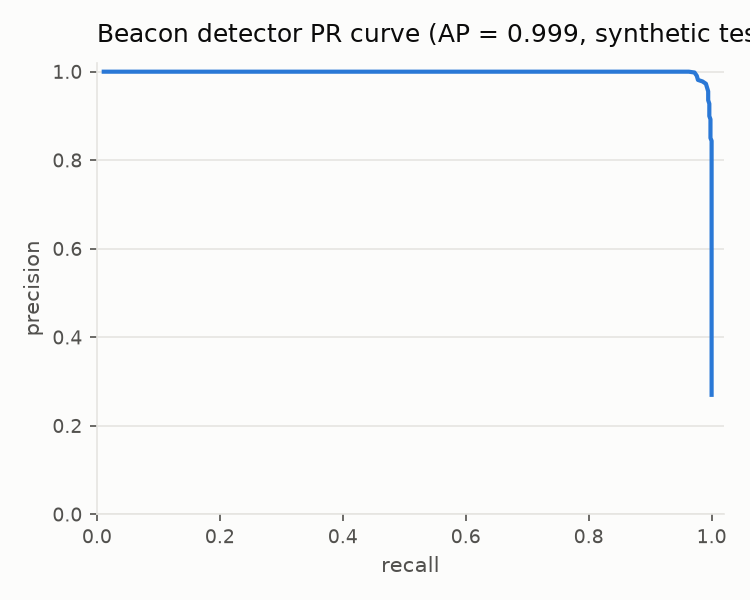
\includegraphics[width=0.55\textwidth]{beacon-detector-PR-curve.png}
\caption{Beacon detector precision--recall curve on the synthetic held-out test set
($n=2000$, AP~$=0.999$). Source: \code{models/beacon\_metrics.json}.}
\label{fig:pr}
\end{figure}

\subsection{LLM backend and record/replay cache}
The LLM client (\code{agent/llm.py}) calls Ollama's generate endpoint with JSON mode, temperature 0
and a fixed seed. Every call is keyed by a SHA-256 of (model, system prompt, prompt) and stored under
\code{cache/<model>/<key>.json} with the response, token counts and latency. In \code{--replay} mode
a cache miss raises an error instead of calling the model, so \code{make smoke} and CI run with no
LLM installed and reproduce the committed numbers exactly. Responses are validated against a small
JSON schema; one automatic repair call is made on violation. Hypotheses naming unknown services are
dropped and unknown fault types become \code{other}, which is how an unseen fault type is reported.

\subsection{Safety layer}
\label{sec:safety}
\Cref{fig:safety} shows the decision flow applied to every planned action. Containment needs
\emph{outbound-compromise} evidence: a beacon finding from the detector when the detector is
running, otherwise an open \code{c2\_beacon} hypothesis; an inbound attack (credential stuffing)
never unlocks containment. Plans are reordered so containment precedes everything else, and a
restart of a host with an open beacon hypothesis is blocked until that host is contained. Execution
is transactional in the sense of STRATUS~\cite{stratus}: observable health is measured before and
after each action (excluding the contained host itself for containment actions, since taking a
compromised host offline is the intended effect) and the action is undone when health drops by more
than 0.15. Containment, rate limits and pool scaling are reversible; restarts and rollbacks are not,
and the record says so.

\begin{figure}[H]
\centering
\adjustbox{max width=\textwidth}{%
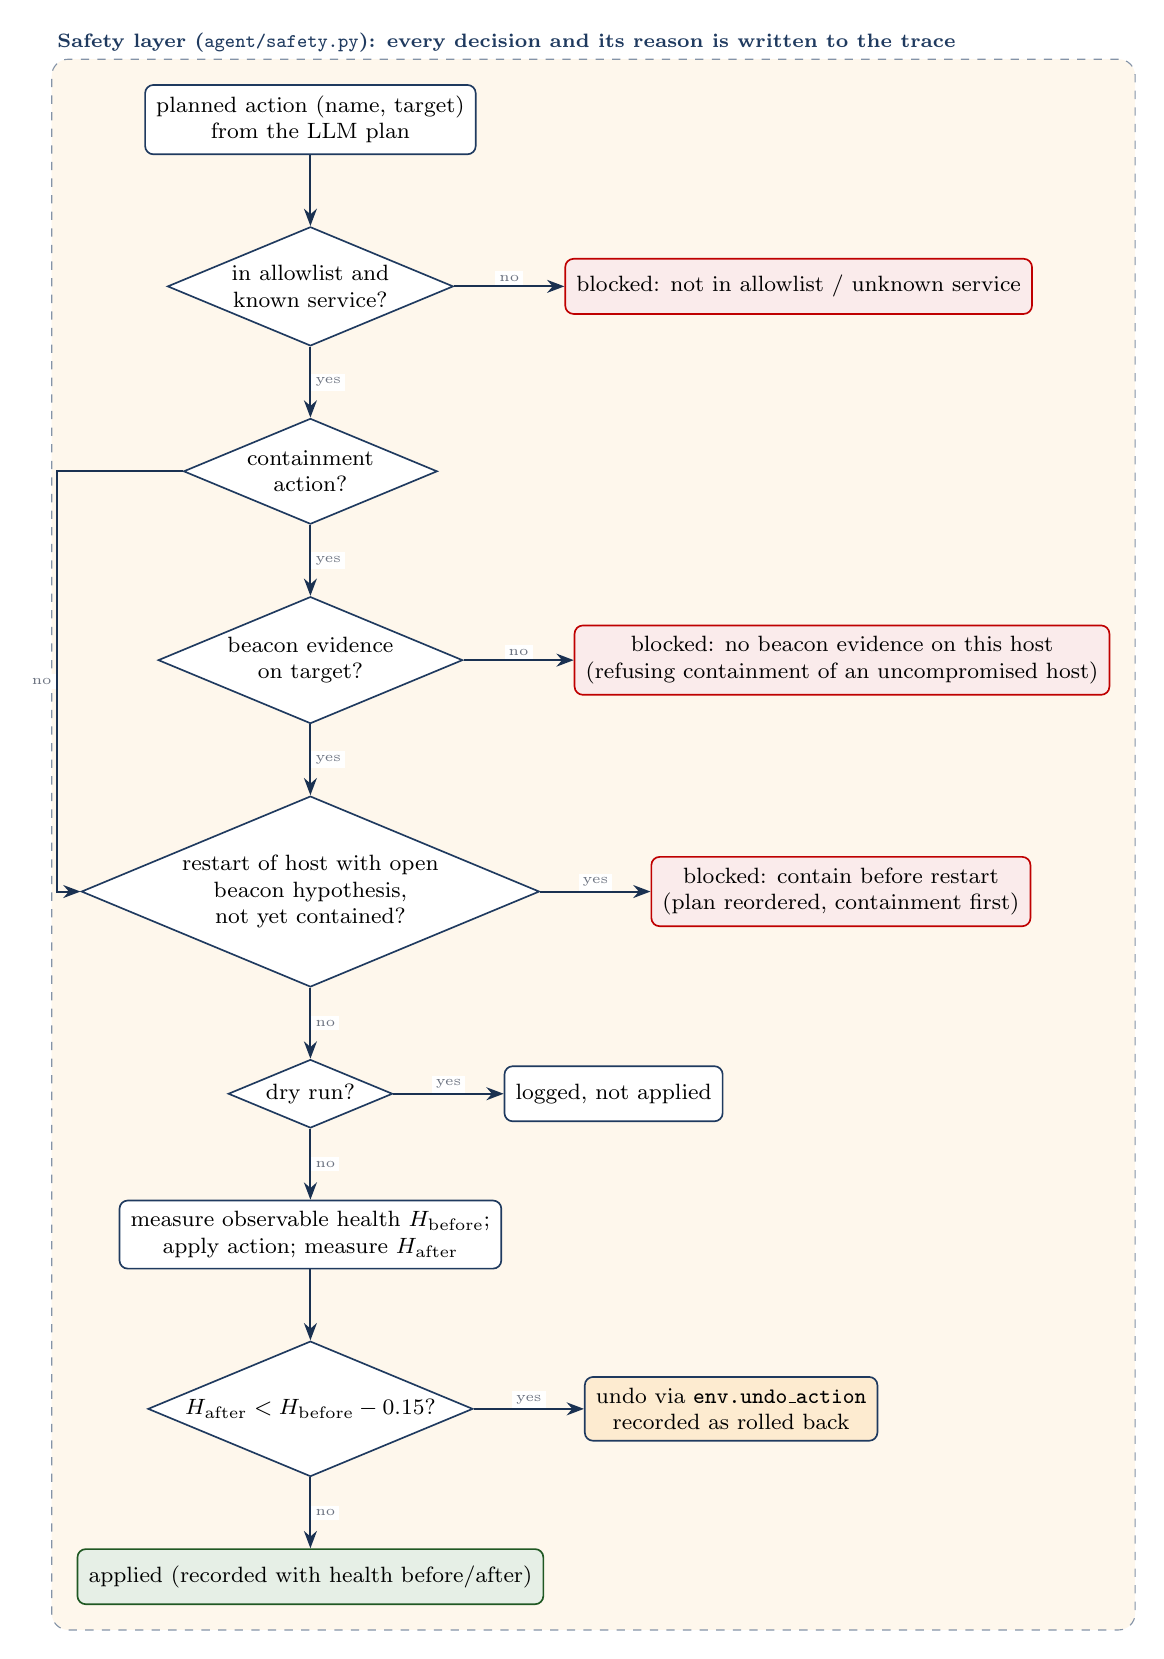
\begin{tikzpicture}[node distance=9mm and 14mm]
  \node[box,minimum width=40mm] (start) {planned action (name, target)\\from the LLM plan};
  \node[decision,below=of start] (d1) {in allowlist and\\known service?};
  \node[decision,below=of d1] (d2) {containment\\action?};
  \node[decision,below=of d2] (d3) {beacon evidence\\on target?};
  \node[decision,below=of d3] (d4) {restart of host with open\\beacon hypothesis,\\not yet contained?};
  \node[decision,below=of d4] (d5) {dry run?};
  \node[box,below=of d5,minimum width=40mm] (apply) {measure observable health $H_{\text{before}}$;\\apply action; measure $H_{\text{after}}$};
  \node[decision,below=of apply] (d6) {$H_{\text{after}} < H_{\text{before}} - 0.15$?};
  \node[good,below=of d6,minimum width=40mm] (ok) {applied (recorded with health before/after)};
  % right column
  \node[bad,right=of d1] (b1) {blocked: not in allowlist / unknown service};
  \node[bad,right=of d3] (b3) {blocked: no beacon evidence on this host\\(refusing containment of an uncompromised host)};
  \node[bad,right=of d4] (b4) {blocked: contain before restart\\(plan reordered, containment first)};
  \node[box,right=of d5] (b5) {logged, not applied};
  \node[safety,right=of d6] (b6) {undo via \code{env.undo\_action}\\recorded as rolled back};
  % edges
  \draw[flow] (start) -- (d1);
  \draw[flow] (d1) -- node[lbl,right] {yes} (d2);
  \draw[flow] (d1) -- node[lbl,above] {no} (b1);
  \draw[flow] (d2) -- node[lbl,right] {yes} (d3);
  \draw[flow] (d2.west) -- ++(-1.6,0) |- node[lbl,pos=0.25,left] {no} (d4.west);
  \draw[flow] (d3) -- node[lbl,above] {no} (b3);
  \draw[flow] (d3) -- node[lbl,right] {yes} (d4);
  \draw[flow] (d4) -- node[lbl,above] {yes} (b4);
  \draw[flow] (d4) -- node[lbl,right] {no} (d5);
  \draw[flow] (d5) -- node[lbl,above] {yes} (b5);
  \draw[flow] (d5) -- node[lbl,right] {no} (apply);
  \draw[flow] (apply) -- (d6);
  \draw[flow] (d6) -- node[lbl,above] {yes} (b6);
  \draw[flow] (d6) -- node[lbl,right] {no} (ok);
  \begin{scope}[on background layer]
    \node[group,fill=safefill!40,fit=(start)(d1)(d6)(ok)(b1)(b3)(b6),
          label={[grouplbl]north west:Safety layer (\code{agent/safety.py}): every decision and its reason is written to the trace}] {};
  \end{scope}
\end{tikzpicture}}
\caption{Safety-layer decision flow for one planned action. With the beacon detector disabled
(ablation, LLM-only) the ``beacon evidence'' test accepts an open \code{c2\_beacon} hypothesis instead.}
\label{fig:safety}
\end{figure}

% =====================================================================
\section{Agent Algorithm}
\label{sec:algo}
% =====================================================================

The loop (\cref{alg:loop}, \cref{fig:fsm}) is MAPE-K with a step budget of 8 iterations and two LLM
calls per iteration. The first call returns ranked hypotheses and up to three targeted checks
(a log grep, a metric window or a flow summary for one service); the checks run deterministically
and their results go into the second call, which returns updated hypotheses and an ordered plan of at
most five actions. A repeated-plan guard re-asks the model once, with an explicit warning, if the
plan is a subset of actions already applied without recovery. Later iterations receive a compact
history of what was done and what verification still flags, so the model changes strategy instead
of repeating itself. The agent may claim ``recovered'' only when the verifier (\cref{alg:verify})
returns no problems; when the budget is exhausted it escalates with the full trace.

\begin{algorithm}[H]
\caption{Sentinel-RX main loop (\code{agent/loop.py::SentinelAgent.run})}
\label{alg:loop}
\begin{algorithmic}[1]
\Require environment $E$, LLM $M$, budget $B=8$, detectors on/off, verify on/off, safety on/off
\State $\mathcal{B} \gets$ \textsc{RememberBaseline}$(E)$ \Comment{first observation: healthy metric and log templates}
\State $\mathcal{H}\gets\emptyset$;\; tried $\gets\emptyset$;\; history $\gets[\,]$
\For{$i = 1,\dots,B$}
  \State $ev \gets$ \textsc{Detect}$(E)$ \Comment{\cref{eq:z,eq:rank,eq:beacon}; grouped per service; raw summary if detectors off}
  \State $(\mathcal{H}', \text{checks}) \gets M.\textsc{Diagnose}(ev, \text{history})$ \Comment{LLM call 1, JSON, $\le3$ checks}
  \State results $\gets$ \textsc{RunChecks}$(E, \text{checks})$ \Comment{deterministic env queries}
  \State $(\mathcal{H}, \text{plan}) \gets M.\textsc{Plan}(\mathcal{H}', \text{results})$ \Comment{LLM call 2, $\le5$ actions}
  \If{keys(plan) $\subseteq$ tried} \Comment{repeated-plan guard}
     \State plan $\gets M.\textsc{Plan}(\mathcal{H}', \text{results}, \text{warning})$
  \EndIf
  \State decisions $\gets$ \textsc{Safety.Screen}(plan, $\mathcal{H}$, beacon hosts) \Comment{\cref{fig:safety}; containment first}
  \ForAll{$d \in$ decisions} \State \textsc{Safety.Execute}$(E, d)$ \Comment{transactional; undo on regression $>0.15$} \EndFor
  \If{verify off} \State claim recovered; \Return \EndIf
  \State \textsc{Wait}$(E,\; 60\,\mathrm{s}$ or $\min(240, 4.5\times\text{beacon interval}))$
  \State problems $\gets$ \textsc{Verify}$(E, \mathcal{B})$ \Comment{\cref{alg:verify}}
  \If{problems $=\emptyset$} \State claim recovered; \Return \EndIf
  \State history $\mathrel{+}=$ (actions, problems);\; tried $\gets$ tried $\cup$ applied actions
\EndFor
\State escalate to a human with the trace
\end{algorithmic}
\end{algorithm}

\begin{algorithm}[H]
\caption{Verification gate (\code{EvidenceBuilder.verify}, \code{Evidence.problems})}
\label{alg:verify}
\begin{algorithmic}[1]
\Require environment $E$, remembered baseline $\mathcal{B}$, time of last action $t_a$, known beacon pairs $K$
\State window $\gets$ telemetry after $t_a + 20\,\mathrm{s}$ \Comment{skip the restart transient}
\State problems $\gets[\,]$
\State add ``services not up'' if any status $\ne$ \code{up};\; add ``health $<0.9$'' if $H<0.9$ (\cref{eq:health})
\State add every metric series whose robust z-score vs.\ $\mathcal{B}$ is $\ge6$ (\cref{eq:z}); add new/surging ERROR, FATAL and WARN templates
\State $F \gets$ \textsc{BeaconDetector}(flows in window, strict: $p\ge0.75$ unknown, $p\ge0.95$ allow-listed/internal)
\ForAll{$(s,d)\in K$} \Comment{pairs flagged during the incident stay suspicious}
  \If{any un-blocked flow $s\to d$ in window and $(s,d)\notin F$} \State $F \gets F \cup \{(s,d)\}$ \EndIf
\EndFor
\State add every $(s,d)\in F$ as ``beacon $s\to d$, $p$, blocked fraction''
\State add ``denied egress attempts (implant still active)'' if blocked flows exist and $F=\emptyset$
\State \Return problems \Comment{empty = the only way to claim ``recovered''}
\end{algorithmic}
\end{algorithm}

\begin{figure}[H]
\centering
\adjustbox{max width=\textwidth}{%
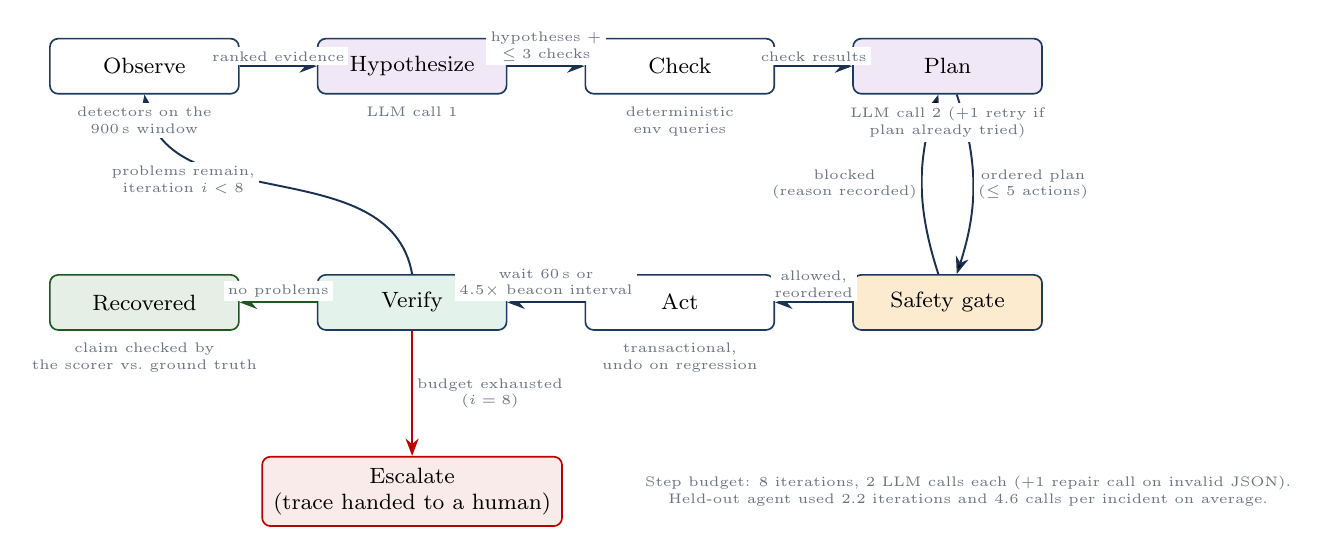
\begin{tikzpicture}
  \node[box,minimum width=24mm] (obs) at (0,0) {Observe};
  \node[llm,minimum width=24mm] (hyp) at (3.4,0) {Hypothesize};
  \node[box,minimum width=24mm] (chk) at (6.8,0) {Check};
  \node[llm,minimum width=24mm] (plan) at (10.2,0) {Plan};
  \node[safety,minimum width=24mm] (safe) at (10.2,-3) {Safety gate};
  \node[box,minimum width=24mm] (act) at (6.8,-3) {Act};
  \node[detector,minimum width=24mm] (ver) at (3.4,-3) {Verify};
  \node[good,minimum width=24mm] (rec) at (0,-3) {Recovered};
  \node[bad,minimum width=24mm] (esc) at (3.4,-5.4) {Escalate\\(trace handed to a human)};
  \draw[flow] (obs) -- node[lbl,above] {ranked evidence} (hyp);
  \draw[flow] (hyp) -- node[lbl,above] {hypotheses +\\$\le3$ checks} (chk);
  \draw[flow] (chk) -- node[lbl,above] {check results} (plan);
  \draw[flow] (plan) edge[bend left=18] node[lbl,right] {ordered plan\\($\le5$ actions)} (safe);
  \draw[flow] (safe) edge[bend left=18] node[lbl,left] {blocked\\(reason recorded)} (plan);
  \draw[flow] (safe) -- node[lbl,above] {allowed,\\reordered} (act);
  \draw[flow] (act) -- node[lbl,above] {wait 60\,s or\\$4.5\times$ beacon interval} (ver);
  \draw[flow,draw=recovered!70!black] (ver) -- node[lbl,above] {no problems} (rec);
  \draw[flow] (ver.north) to[out=100,in=-80] node[lbl,left,pos=0.55] {problems remain,\\iteration $i<8$} (obs.south);
  \draw[flow,draw=attack] (ver) -- node[lbl,right] {budget exhausted\\($i=8$)} (esc);
  \node[lbl,below=1mm of obs] {detectors on the\\900\,s window};
  \node[lbl,below=1mm of hyp] {LLM call 1};
  \node[lbl,below=1mm of chk] {deterministic\\env queries};
  \node[lbl,below=1mm of plan] {LLM call 2 (+1 retry if\\plan already tried)};
  \node[lbl,below=1mm of act] {transactional,\\undo on regression};
  \node[lbl,below=1mm of rec] {claim checked by\\the scorer vs.\ ground truth};
  \node[lbl,anchor=west] at (6.3,-5.4) {Step budget: 8 iterations, 2 LLM calls each (+1 repair call on invalid JSON).\\Held-out agent used 2.2 iterations and 4.6 calls per incident on average.};
\end{tikzpicture}}
\caption{Agent loop as a state machine. Hypothesize and Plan are the only LLM calls; everything else is deterministic.}
\label{fig:fsm}
\end{figure}

\begin{figure}[H]
\centering
\adjustbox{max width=\textwidth}{%
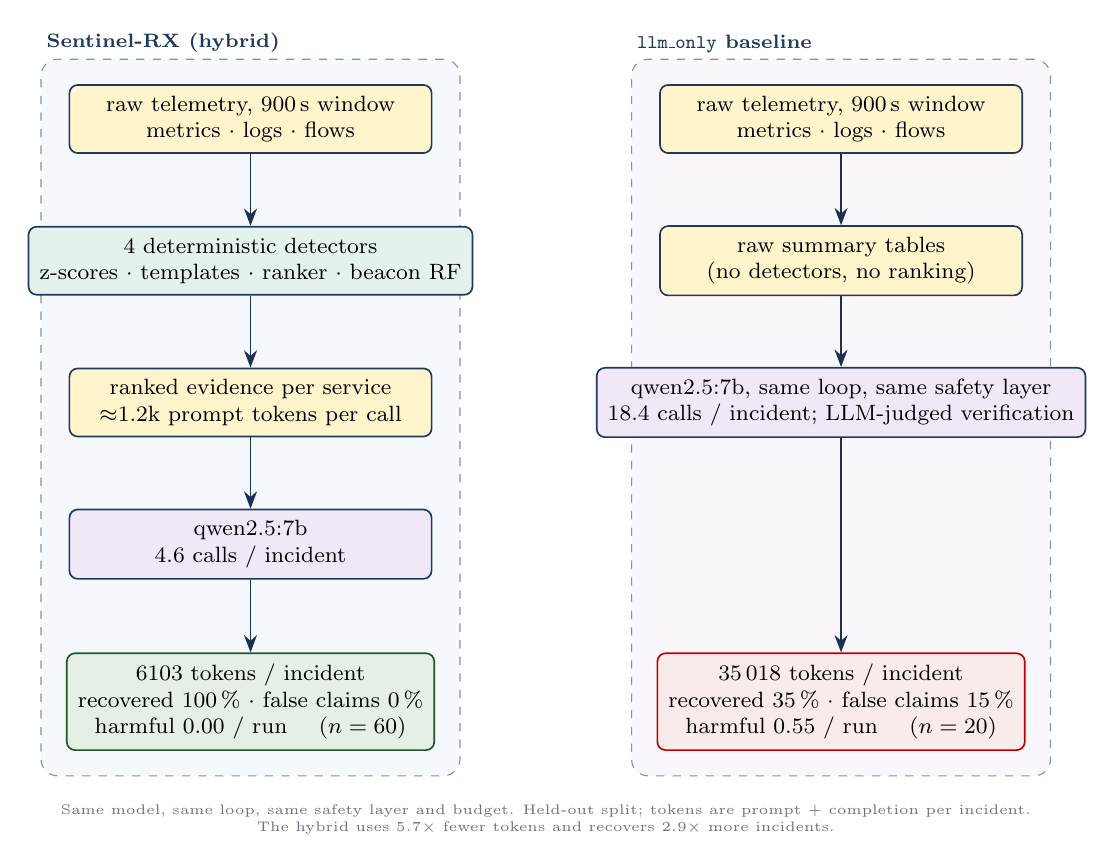
\begin{tikzpicture}
  % ---- left: hybrid ----
  \node[output,minimum width=46mm] (rawL) at (0,0) {raw telemetry, 900\,s window\\metrics $\cdot$ logs $\cdot$ flows};
  \node[detector,minimum width=46mm] (detL) at (0,-1.8) {4 deterministic detectors\\z-scores $\cdot$ templates $\cdot$ ranker $\cdot$ beacon RF};
  \node[output,minimum width=46mm] (evL) at (0,-3.6) {ranked evidence per service\\$\approx$1.2k prompt tokens per call};
  \node[llm,minimum width=46mm] (llmL) at (0,-5.4) {qwen2.5:7b\\4.6 calls / incident};
  \node[good,minimum width=46mm] (outL) at (0,-7.4) {\num{6103} tokens / incident\\recovered \pct{100} $\cdot$ false claims \pct{0}\\harmful 0.00 / run \quad ($n=60$)};
  \draw[flow] (rawL) -- (detL); \draw[flow] (detL) -- (evL); \draw[flow] (evL) -- (llmL); \draw[flow] (llmL) -- (outL);
  \begin{scope}[on background layer]
    \node[group,fit=(rawL)(outL),label={[grouplbl]north west:Sentinel-RX (hybrid)}] (gL) {};
  \end{scope}
  % ---- right: llm only ----
  \node[output,minimum width=46mm] (rawR) at (7.5,0) {raw telemetry, 900\,s window\\metrics $\cdot$ logs $\cdot$ flows};
  \node[output,minimum width=46mm] (sumR) at (7.5,-1.8) {raw summary tables\\(no detectors, no ranking)};
  \node[llm,minimum width=46mm] (llmR) at (7.5,-3.6) {qwen2.5:7b, same loop, same safety layer\\18.4 calls / incident; LLM-judged verification};
  \node[bad,minimum width=46mm] (outR) at (7.5,-7.4) {\num{35018} tokens / incident\\recovered \pct{35} $\cdot$ false claims \pct{15}\\harmful 0.55 / run \quad ($n=20$)};
  \draw[flow] (rawR) -- (sumR); \draw[flow] (sumR) -- (llmR); \draw[flow] (llmR) -- (outR);
  \begin{scope}[on background layer]
    \node[group,fill=llmfill!40,fit=(rawR)(outR),label={[grouplbl]north west:\code{llm\_only} baseline}] (gR) {};
  \end{scope}
  \node[lbl,align=center] at (3.75,-8.9) {Same model, same loop, same safety layer and budget. Held-out split; tokens are prompt + completion per incident.\\The hybrid uses $5.7\times$ fewer tokens and recovers $2.9\times$ more incidents.};
\end{tikzpicture}}
\caption{Hybrid design versus the raw-telemetry variant of the same loop. Detectors compress and rank
before the model reads anything; the token and outcome numbers are the held-out results of \cref{sec:results}.}
\label{fig:hybrid}
\end{figure}

% =====================================================================
\section{Evaluation Methodology}
\label{sec:eval}
% =====================================================================

\subsection{Scenario generation and split discipline}
\code{scenarios/generate.py} produces YAML scenarios deterministically from one master seed.
A scenario is a list of (type, target, start tick, parameters) faults with distinct types and distinct
targets; parameters (leak rate, pool ramp, injected latency, beacon interval 25--60\,s with
10--35\,\% jitter, destination) are drawn per scenario. The \textbf{dev} split has 30 scenarios
(10 single-fault, 12 two-fault, 8 three-fault); the \textbf{held-out} split has 20 (4/9/7). Every
held-out scenario uses a fault combination (sorted \code{type@target} key) that never occurs in dev,
multi-fault held-out scenarios use a multiset of fault \emph{types} never seen in dev, and the two
splits draw seeds from disjoint ranges. \code{dns\_failure} never appears outside the unseen-fault
set. \code{tests/test\_scenarios.py} asserts all of this against the committed YAML.

The runner refuses to touch any non-dev split without \code{--final} and appends every such run,
with its git revision, to \code{results/heldout\_runs.log}, which is committed. All agent tuning
(\cref{sec:audit}, \code{docs/RESULTS.md}) happened on dev; the agent, detectors, prompts,
simulator and scorer were then frozen under the tag \code{v1-frozen} and every held-out,
perturbation, ablation and small-model number in this report was produced after that tag.

\begin{figure}[H]
\centering
\adjustbox{max width=\textwidth}{%
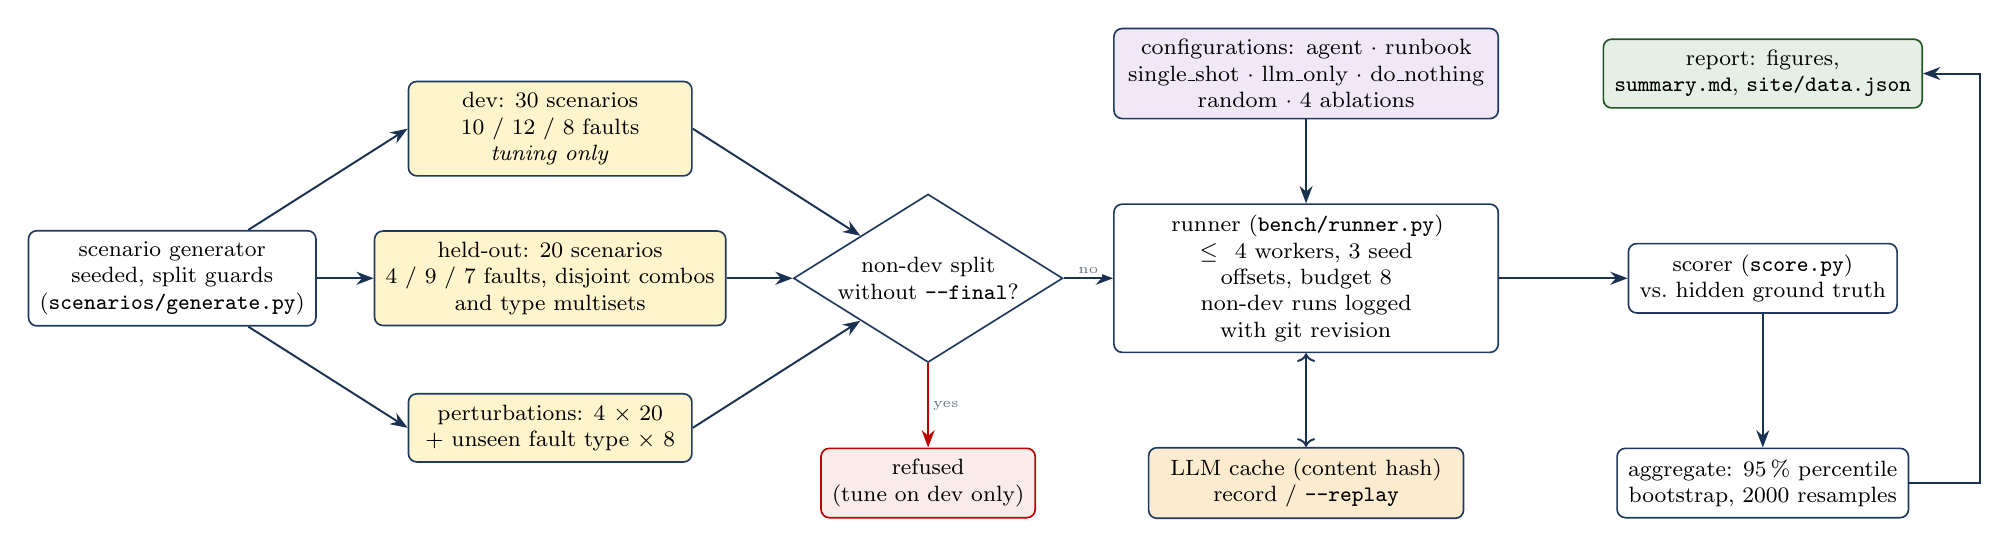
\begin{tikzpicture}
  \node[box,minimum width=30mm] (gen) at (0,0) {scenario generator\\seeded, split guards\\(\code{scenarios/generate.py})};
  \node[output,minimum width=36mm] (dev) at (4.8,1.9) {dev: 30 scenarios\\10 / 12 / 8 faults\\\emph{tuning only}};
  \node[output,minimum width=36mm] (held) at (4.8,0) {held-out: 20 scenarios\\4 / 9 / 7 faults, disjoint combos\\and type multisets};
  \node[output,minimum width=36mm] (pert) at (4.8,-1.9) {perturbations: 4 $\times$ 20\\+ unseen fault type $\times$ 8};
  \draw[flow] (gen) -- (dev.west); \draw[flow] (gen) -- (held.west); \draw[flow] (gen) -- (pert.west);
  \node[decision,aspect=1.6] (guard) at (9.6,0) {non-dev split\\without \code{--final}?};
  \draw[flow] (dev.east) -- (guard.north west); \draw[flow] (held.east) -- (guard.west); \draw[flow] (pert.east) -- (guard.south west);
  \node[bad] (refuse) at (9.6,-2.6) {refused\\(tune on dev only)};
  \draw[flow,draw=attack] (guard) -- node[lbl,right] {yes} (refuse);
  \node[box,text width=46mm] (run) at (14.4,0) {runner (\code{bench/runner.py})\\$\le4$ workers, 3 seed offsets, budget 8\\non-dev runs logged with git revision};
  \draw[flow] (guard) -- node[lbl,above] {no} (run);
  \node[llm,text width=46mm] (cfg) at (14.4,2.6) {configurations: agent $\cdot$ runbook\\single\_shot $\cdot$ llm\_only $\cdot$ do\_nothing\\random $\cdot$ 4 ablations};
  \draw[flow] (cfg) -- (run);
  \node[safety,minimum width=40mm] (cache) at (14.4,-2.6) {LLM cache (content hash)\\record / \code{--replay}};
  \draw[flow,<->] (run) -- (cache);
  \node[box,minimum width=28mm] (score) at (20.2,0) {scorer (\code{score.py})\\vs.\ hidden ground truth};
  \draw[flow] (run) -- (score);
  \node[box,minimum width=28mm] (agg) at (20.2,-2.6) {aggregate: 95\,\% percentile\\bootstrap, 2000 resamples};
  \draw[flow] (score) -- (agg);
  \node[good,minimum width=28mm] (rep) at (20.2,2.6) {report: figures,\\\code{summary.md}, \code{site/data.json}};
  \draw[flow] (agg.east) -- ++(0.9,0) |- (rep.east);
\end{tikzpicture}}
\caption{Evaluation pipeline. Nothing outside dev can be run without the \code{--final} flag, and every such run is logged with its git revision in \code{results/heldout\_runs.log}; per-scenario traces flow from the runner to the scorer.}
\label{fig:pipeline}
\end{figure}

\subsection{Perturbations}
Perturbations wrap the environment at the observation layer, so the simulator and ground truth are
untouched: \textbf{noisy logs} inject \pct{80} extra benign lines; \textbf{missing metrics} drop
values; \textbf{renamed services} present the agent with a different service vocabulary (the scorer
maps hypotheses back); \textbf{timestamp jitter} adds Gaussian clock skew ($\sigma=2$\,s) to log and flow
timestamps; \textbf{unseen fault} injects \code{dns\_failure}, which the agent's taxonomy does not
describe. A \textbf{smaller model} run swaps \code{qwen2.5:7b} for \code{qwen2.5:1.5b}.

\subsection{Baselines and ablations}
\begin{itemize}
  \item \textbf{runbook}: static if-symptom-then-action threshold rules and log greps, looping until no
        rule fires; given a naive ``any egress to an unknown destination'' rule so it is not strawmanned on security.
  \item \textbf{single\_shot}: one LLM call on a telemetry summary, acts, no loop, no verification.
  \item \textbf{llm\_only}: the full loop and safety layer but no detectors; the prompt carries a raw
        telemetry summary and verification is LLM-judged.
  \item \textbf{do\_nothing}: never acts; claims recovery iff observable health $\ge0.9$.
  \item \textbf{random}: 1--3 random allow-listed actions on random services per iteration; claims
        recovery when health $\ge0.9$. Together with do\_nothing it is a permanent sanity floor: any
        scenario these recover is a scenario where the recovery check is broken.
  \item \textbf{Ablations}: \code{no\_verify} (claims recovery after acting), \code{no\_loop} (one
        iteration), \code{no\_beacon} (beacon detector off), \code{no\_safety} (no allowlist,
        ordering or rollback).
\end{itemize}

\subsection{Metrics}
Let $T$ be the set of injected (service, type) faults, $R$ the agent's final non-refuted hypotheses
ranked by confidence, $A$ the applied actions, and $A_{\text{eff}}\subseteq A$ those the simulator
recorded as resolving or containing a fault.
\begin{align}
  \text{top-}k &= \mathbf{1}\big[\exists\, h\in R_{1..k},\, t\in T:\; h=t\big], \notag\\
  \text{recall} &= \frac{|\{t\in T:\exists h\in R_{\text{diag}}, h=t\}|}{|T|}, \notag\\
  \text{recovered} &= \mathbf{1}[\text{all faults resolved, all services up, } H\ge0.9 \text{ for 2 ticks}], \notag\\
  \text{false recovery} &= \mathbf{1}[\text{claimed} \wedge \neg\text{recovered}], \notag\\
  \text{harmful} &= \#\{\text{restarts before containment}\} + \#\{\text{containments of uncompromised hosts}\}, \notag\\
  \text{unnecessary} &= |A| - |A_{\text{eff}}|, \qquad
  \text{action precision} = \frac{|A_{\text{eff}}|}{|A|},
  \label{eq:metrics}
\end{align}
plus isolated-before-restart (1 if no beacon was reinfected), rolled-back actions, LLM calls and
tokens (prompt + completion), wall-clock and time to recovery. Per-run scores are averaged over
(scenario $\times$ seed offset) runs and reported with \pct{95} percentile-bootstrap confidence
intervals (2000 resamples, fixed RNG seed). Headline configurations use 3 seed offsets per held-out
scenario ($n=60$); \code{llm\_only}, perturbations, ablations and the small-model run use 1
($n=20$; 8 for the unseen fault) because of the laptop time budget (\cref{sec:limits}).

% =====================================================================
\section{Results}
\label{sec:results}
% =====================================================================

\subsection{Held-out benchmark}
\Cref{tab:heldout} is the headline table; \cref{fig:byconfig} plots the four main metrics. Top-3 root-cause accuracy is \pct{95} for the agent and the runbook, \pct{78} for single\_shot and \pct{60} for llm\_only.
All configurations run the same 20 held-out scenarios with the same 8-iteration budget; agent,
runbook, single\_shot, do\_nothing and random use 3 seed offsets, llm\_only 1.

\begin{table}[H]
\centering\footnotesize
\caption{Held-out results (\code{qwen2.5:7b}, 20 scenarios; $n$ = runs). Means with \pct{95}
bootstrap CIs. Harmful and unnecessary actions are counts per run. Source: \code{results/summary.md}.}
\label{tab:heldout}
\setlength{\tabcolsep}{4pt}
\adjustbox{max width=\textwidth}{%
\begin{tabular}{l r r r r r r r r r}
\toprule
config & top-1 & recall & recovered & false ``rec.'' & harmful / run & action prec. & calls & tokens & $n$ \\
\midrule
\rowcolor{groupfill}\textbf{agent} & \textbf{92} \ci{83}{98} & \textbf{82} \ci{74}{89} & \textbf{100} \ci{100}{100} & \textbf{0} \ci{0}{0} & \textbf{0.00} & \textbf{81} \ci{74}{88} & 4.6 & \num{6103} & 60 \\
runbook & 87 \ci{78}{95} & 81 \ci{74}{87} & 45 \ci{32}{58} & 5 \ci{0}{12} & 0.00 & 74 \ci{68}{80} & 0 & 0 & 60 \\
single\_shot & 63 \ci{50}{75} & 50 \ci{41}{59} & 30 \ci{20}{42} & 70 \ci{58}{80} & 0.27 \ci{0.15}{0.38} & 37 \ci{30}{43} & 1.0 & \num{2421} & 60 \\
llm\_only & 35 \ci{15}{55} & 44 \ci{28}{61} & 35 \ci{15}{55} & 15 \ci{0}{30} & 0.55 \ci{0.15}{1.05} & 25 \ci{13}{39} & 18.4 & \num{35018} & 20 \\
do\_nothing & 0 & 0 & 0 & 0 & 0.00 & n/a & 0 & 0 & 60 \\
random & 0 & 0 & 0 & 10 \ci{3}{18} & 3.45 \ci{2.92}{3.98} & 5 \ci{4}{7} & 0 & 0 & 60 \\
\bottomrule
\end{tabular}}
\end{table}

\begin{figure}[H]
\centering
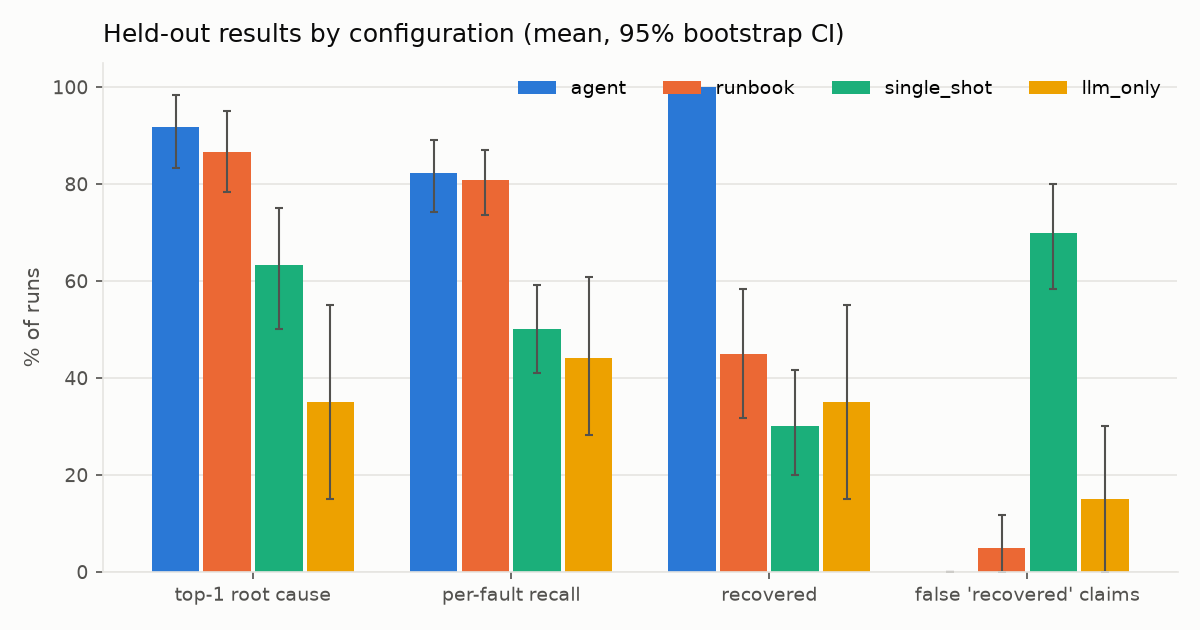
\includegraphics[width=0.9\textwidth]{results-by-config.png}
\caption{Held-out top-1, per-fault recall, recovery and false-recovery rate per configuration with
\pct{95} bootstrap CIs (\code{make report}).}
\label{fig:byconfig}
\end{figure}

\begin{keyfinding}{recovery and honesty (G1, G3)}
The agent recovers \pct{100} of held-out incidents (CI [100, 100], $n=60$) with \pct{0} false
claims. The runbook diagnoses nearly as well (top-1 \pct{87} vs.\ \pct{92}) but recovers only
\pct{45}: its thresholds are literally the fault definitions, yet it cannot tell symptom from cause
and never eradicates a contained implant. The single-shot LLM claims recovery falsely in \pct{70} of
runs because nothing checks its claim. The two sanity floors recover \pct{0}, so the recovery check
gives nothing away.
\end{keyfinding}

\paragraph{Concurrency.} \Cref{tab:byn} and \cref{fig:byn} break the held-out results down by the
number of concurrent faults. The agent's recovery rate is flat at \pct{100} from one to three faults;
every baseline degrades with concurrency. The agent's top-1 is \emph{lowest} on single-fault scenarios
(\pct{75}, 12 runs): the misses are type confusions where the fix coincides (a cache latency injection
labelled \code{cache\_failure} and resolved by a restart), which count as top-1 misses but not as
recovery misses by design.

\begin{table}[H]
\centering\small
\caption{Held-out recovered / top-1 by number of concurrent faults (runs per cell: 12 / 27 / 21 for
3-seed configurations, 4 / 9 / 7 for llm\_only).}
\label{tab:byn}
\begin{tabular}{l rr rr rr}
\toprule
 & \multicolumn{2}{c}{1 fault} & \multicolumn{2}{c}{2 faults} & \multicolumn{2}{c}{3 faults} \\
\cmidrule(lr){2-3}\cmidrule(lr){4-5}\cmidrule(lr){6-7}
config & recovered & top-1 & recovered & top-1 & recovered & top-1 \\
\midrule
\rowcolor{groupfill}\textbf{agent} & \pct{100} & \pct{75} & \pct{100} & \pct{93} & \pct{100} & \pct{100} \\
runbook & \pct{75} & \pct{50} & \pct{37} & \pct{93} & \pct{38} & \pct{100} \\
single\_shot & \pct{75} & \pct{50} & \pct{33} & \pct{67} & \pct{0} & \pct{67} \\
llm\_only & \pct{100} & \pct{50} & \pct{22} & \pct{33} & \pct{14} & \pct{29} \\
\bottomrule
\end{tabular}
\end{table}

\begin{figure}[H]
\centering
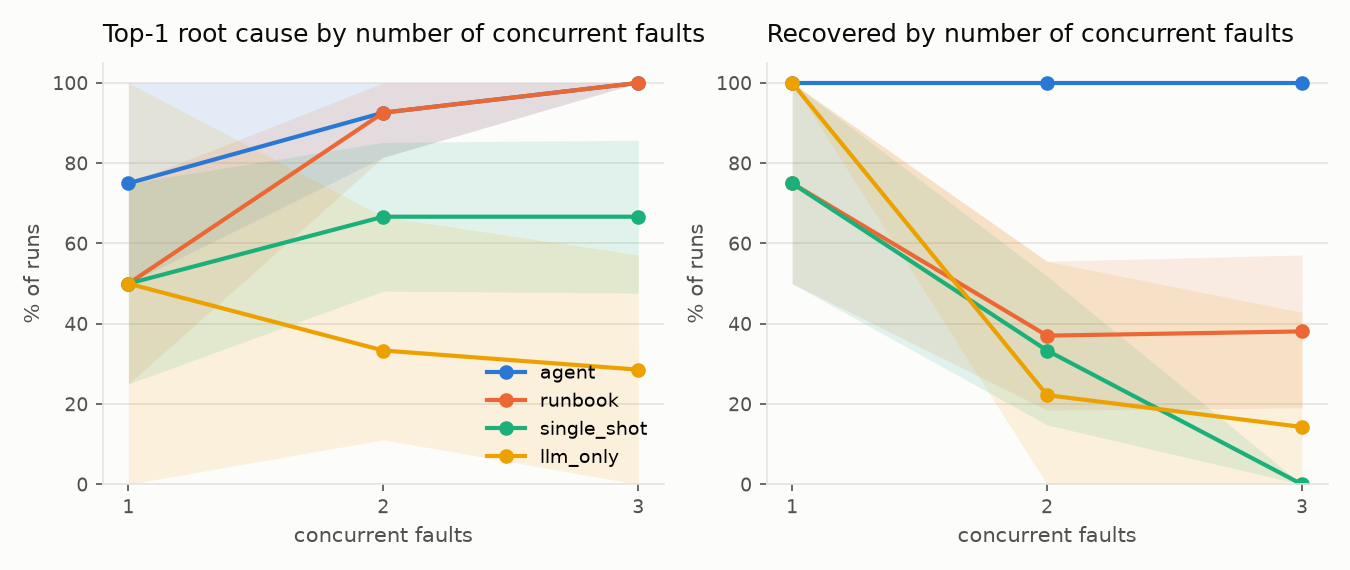
\includegraphics[width=0.95\textwidth]{accuracy-by-number-of-concurrent-faults.png}
\caption{Top-1 root cause and recovery versus number of concurrent faults, held-out split, shaded \pct{95} CIs.}
\label{fig:byn}
\end{figure}

\paragraph{Security subset.} 9 of the 20 held-out scenarios contain a security fault (27 runs with 3
seeds; 21 of them with a C2 beacon). On them the agent recovers \pct{100} with isolated-before-restart \pct{100} and 0 harmful
actions; the runbook recovers \pct{33} (it blocks egress but never eradicates); single\_shot recovers
\pct{15} with isolated-before-restart \pct{38} and 0.48 harmful actions per run; llm\_only (1 seed, 9 runs) recovers
\pct{11} with 1.11 harmful actions per run; random commits 3.04 harmful actions per run.

\begin{keyfinding}{security-aware ordering (G2)}
Across the 27 held-out runs with a security fault (21 with a C2 beacon) the agent never restarted a
compromised host before containing it and never contained an uncompromised one. single\_shot (no
safety layer) and llm\_only (no beacon detector) did so routinely (0.48 and 1.11 harmful actions
per run over 27 and 9 runs), and a random
walk over the same eight actions is harmful 3.04 times per run: the action space is dangerous by
default, and the safety layer, not the model, is what makes it safe.
\end{keyfinding}

\subsection{Robustness}
\Cref{tab:robust} and \cref{fig:robust} report the agent on the held-out variants (1 seed).

\begin{table}[H]
\centering\small
\caption{Agent under perturbations (held-out variants, 1 seed). Change is in recovered percentage points vs.\ the full agent on the same seed of the clean held-out split.}
\label{tab:robust}
\begin{tabular}{l r r r r r r}
\toprule
perturbation & top-1 & recovered & false ``rec.'' & harmful/run & $\Delta$ recovered & $n$ \\
\midrule
\rowcolor{groupfill}clean held-out (3 seeds) & \pct{92} & \pct{100} & \pct{0} & 0.00 & -- & 60 \\
noisy\_logs (+\pct{80} benign lines) & \pct{95} & \pct{100} & \pct{0} & 0.00 & $0$ & 20 \\
missing\_metrics & \pct{90} & \pct{95} & \pct{0} & 0.00 & $-5$ & 20 \\
renamed\_services & \pct{90} & \pct{100} & \pct{0} & 0.00 & $0$ & 20 \\
timestamp\_jitter ($\sigma=2$\,s) & \pct{90} & \pct{100} & \pct{0} & 0.00 & $0$ & 20 \\
unseen\_fault (dns\_failure) & \pct{62} & \pct{100} & \pct{0} & 0.00 & $0$ & 8 \\
smaller LLM (qwen2.5:1.5b) & \pct{40} & \pct{50} & \pct{0} & 0.00 & $-50$ & 20 \\
\bottomrule
\end{tabular}
\end{table}

\begin{figure}[H]
\centering
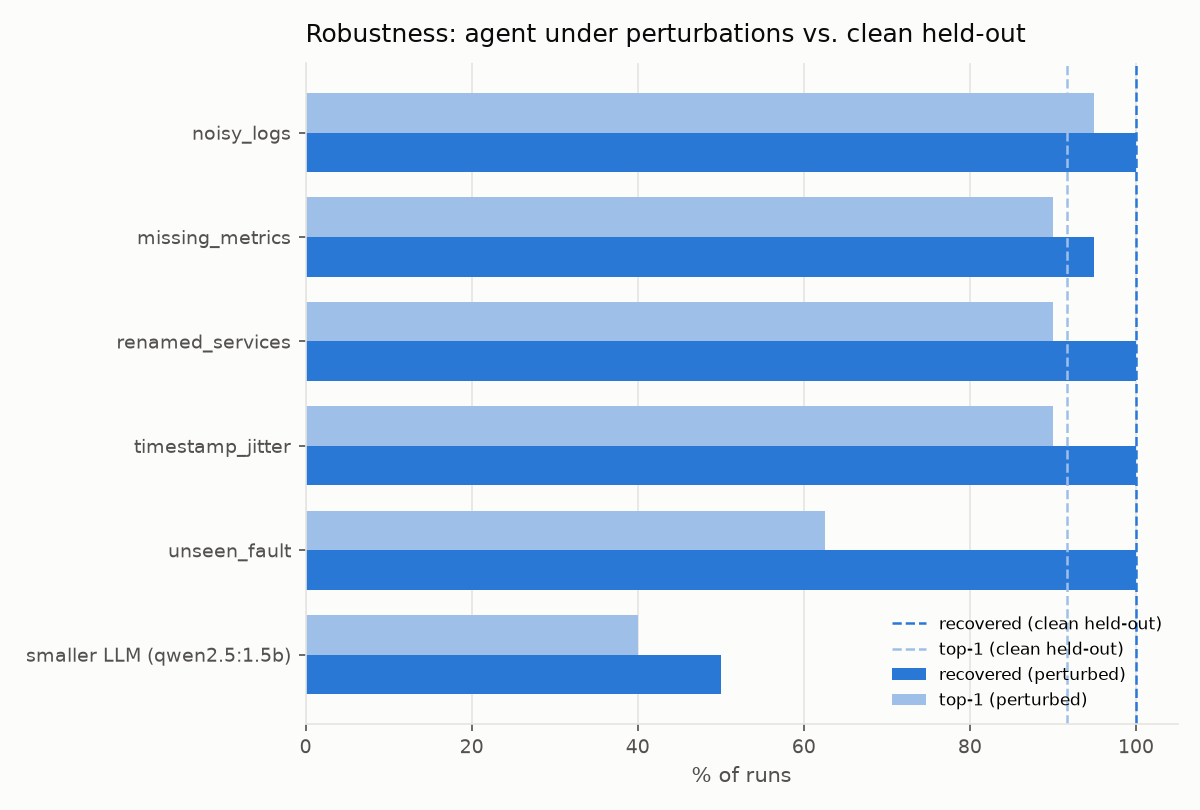
\includegraphics[width=0.85\textwidth]{robustness-drop.png}
\caption{Robustness: agent under each perturbation versus clean held-out.}
\label{fig:robust}
\end{figure}

\begin{keyfinding}{robustness and the unseen fault (G5)}
Recovery stays at \pct{95}--\pct{100} under all four telemetry perturbations. On the fault type the
taxonomy does not describe, the agent never names it (per-fault recall 0/8; the \pct{62} top-1 on
that split comes from the known co-fault) but it localizes the faulty service (\pct{94}) and every
incident is still recovered, because the remediation it reaches for (rollback or restart of the
anomalous host) is one of that fault's accepted fixes and the verifier keeps it looping until the
symptoms are gone. This shows safe degradation on an unknown fault, not diagnosis of it. The 1.5B model loses half the recoveries (\pct{50}, 17.8 calls per run)
yet still makes \pct{0} false claims and 0 harmful actions.
\end{keyfinding}

\subsection{Ablations}
\begin{table}[H]
\centering\small
\caption{Ablations on held-out (1 seed, $n=20$ each). Delta in parentheses is ablated minus the full agent on the same seed.}
\label{tab:ablate}
\begin{tabular}{l r r r r r r}
\toprule
ablation & top-1 & recovered & false ``rec.'' & harmful/run & unnecessary/run & calls \\
\midrule
\rowcolor{groupfill}full agent & \pct{92} & \pct{100} & \pct{0} & 0.00 & 1.18 & 4.6 \\
no\_verify & \pct{80} ($-10$) & \pct{20} ($-80$) & \pct{80} ($+80$) & 0.00 & 0.60 & 2.0 \\
no\_loop & \pct{80} ($-10$) & \pct{20} ($-80$) & \pct{0} & 0.00 & 0.60 & 2.0 \\
no\_beacon & \pct{85} ($-5$) & \pct{50} ($-50$) & \pct{35} ($+35$) & 0.05 ($+0.05$) & 2.75 ($+1.75$) & 6.2 \\
no\_safety & \pct{90} ($0$) & \pct{100} ($0$) & \pct{0} & 0.60 ($+0.60$) & 2.05 ($+1.05$) & 4.8 \\
\bottomrule
\end{tabular}
\end{table}

\begin{figure}[H]
\centering
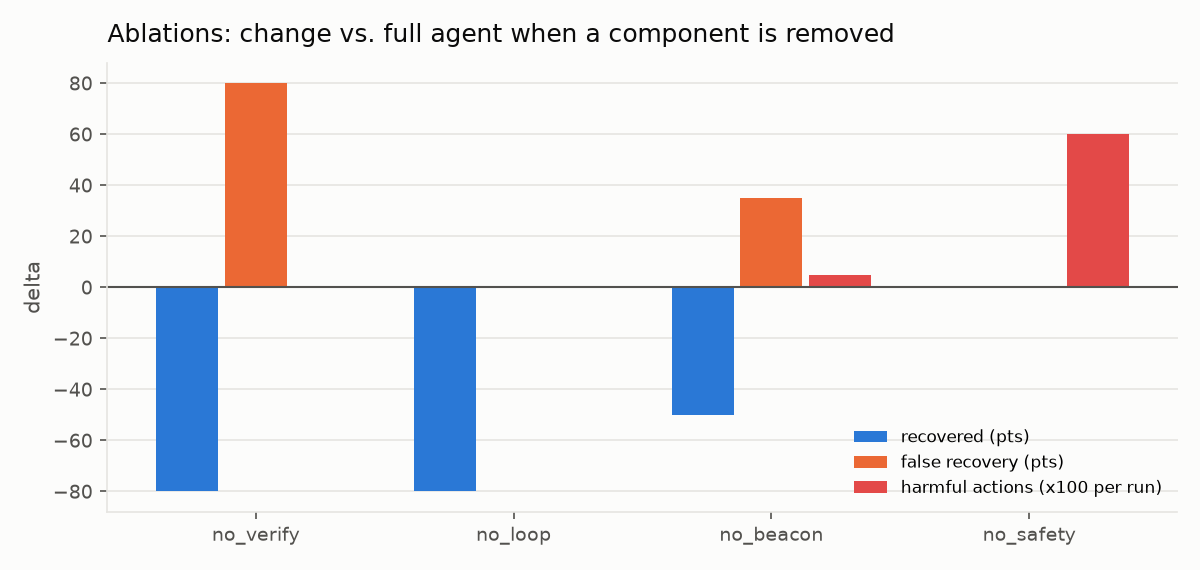
\includegraphics[width=0.85\textwidth]{ablation-deltas.png}
\caption{Ablation deltas relative to the full agent (held-out, 1 seed).}
\label{fig:ablate}
\end{figure}

\begin{keyfinding}{each component protects a different metric}
\code{no\_verify} and \code{no\_loop} produce identical actions (one iteration, 2 calls) and the
same \pct{20} recovery; the only difference is that \code{no\_verify} \emph{claims} success in
\pct{80} of runs while \code{no\_loop} escalates honestly. Verification is therefore worth 80 points
of false claims, the loop 80 points of recovery. Without the beacon detector the remaining detectors
still diagnose well (top-1 \pct{85}) but recovery halves and false claims appear, because the
verifier can no longer see the implant and no security scenario is recovered (0 of 9). Without the
safety layer recovery is unchanged, but 0.60 harmful actions per run appear: the model does restart
compromised hosts when nothing stops it.
\end{keyfinding}

\subsection{Cost}
\begin{table}[H]
\centering\small
\caption{Cost per incident on held-out (means). Wall-clock is the agent's own run time per incident on the laptop; ``whole command'' is the elapsed time of the evaluation command that produced the result file.}
\label{tab:cost}
\adjustbox{max width=\textwidth}{%
\begin{tabular}{l r r r r r r}
\toprule
config & LLM calls & tokens & iterations & actions & wall-clock / incident & whole command \\
\midrule
\rowcolor{groupfill}agent (3 seeds) & 4.6 & \num{6103} & 2.2 & 3.7 & 190\,s & 63\,min \\
single\_shot (3 seeds) & 1.0 & \num{2421} & 1.0 & 2.9 & 85\,s & 29\,min \\
llm\_only (1 seed) & 18.4 & \num{35018} & 5.4 & 9.8 & 816\,s & 95\,min \\
agent, qwen2.5:1.5b (1 seed) & 17.8 & \num{29659} & 6.0 & 6.7 & 394\,s & 45\,min \\
runbook / do\_nothing / random & 0 & 0 & 2.5 / 8 / 7.6 & 2.5 / 0 / 13.8 & $<0.02$\,s & $<2$\,s \\
\bottomrule
\end{tabular}}
\end{table}

\begin{figure}[H]
\centering
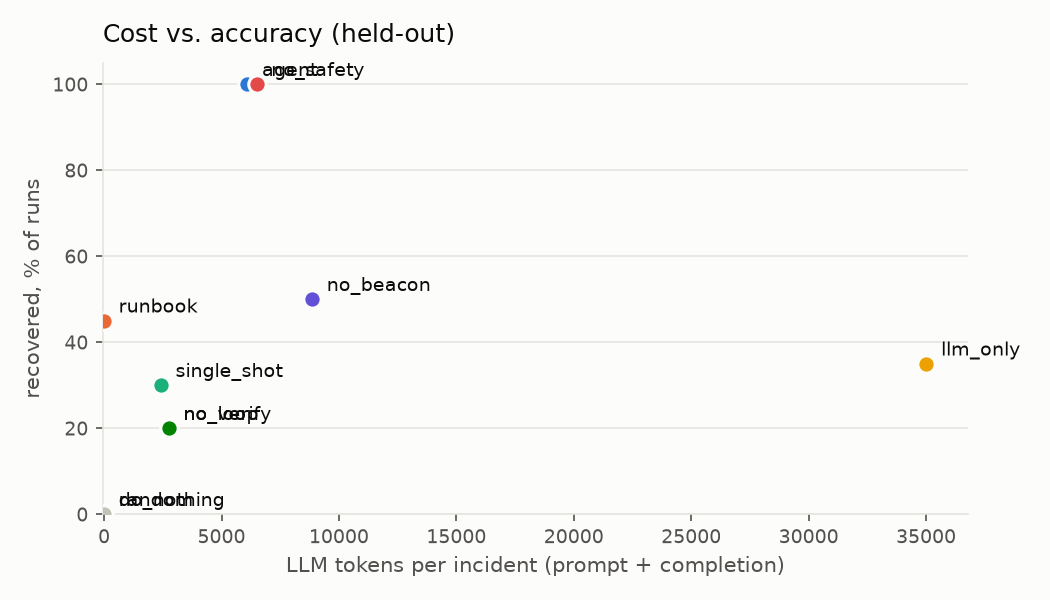
\includegraphics[width=0.75\textwidth]{cost-vs-accuracy.png}
\caption{Tokens per incident versus recovery rate, held-out split, all configurations and ablations.}
\label{fig:cost}
\end{figure}

\begin{keyfinding}{cost of the agent (G4)}
The hybrid agent needs \num{6103} tokens and 4.6 calls per incident on a local 7B model; the same
loop reading raw telemetry needs $5.7\times$ more tokens and $4\times$ more calls to recover
$2.9\times$ fewer incidents. Compressing and ranking evidence before the model reads it is both the
cheapest and the most accurate design tested. The smaller model is not cheaper either: it burns
\num{29659} tokens looping on wrong plans.
\end{keyfinding}

\subsection{Live demonstration}
\Cref{fig:timeline} reconstructs the recorded \code{make demo-live} run from
\code{results/demo\_live\_trace.json} and \code{results/demo\_live\_console.txt}. Three faults were
injected concurrently on real processes after a 35\,s baseline: a memory leak on \code{api}
($\approx$6\,MB/s), a connection-pool hold on \code{db}, and a C2 beacon on \code{worker} every
$\approx$4\,s $\pm$\pct{20} to a local sinkhole. Health fell from 1.00 to 0.10. The model's first
plan targeted the wrong host for the pool (``api: db\_conn\_exhaustion'') and tried to restart
\code{worker}; the safety layer blocked that restart because the beacon detector had flagged
\code{worker} ($p=0.82$). Verification refused ``recovered'' twice, each time naming the live beacon.
In the third iteration the model blocked \code{worker}'s egress and only then restarted it. The live
system's own ground truth afterwards: no active faults, restart-before-containment $=0$, 97 beacon
hits on the sinkhole before containment, final health 1.00. The agent used 6 LLM calls and
\num{9058} tokens; its run took 370\,s of which 292\,s were model latency.

\begin{figure}[H]
\centering
\adjustbox{max width=\textwidth}{%
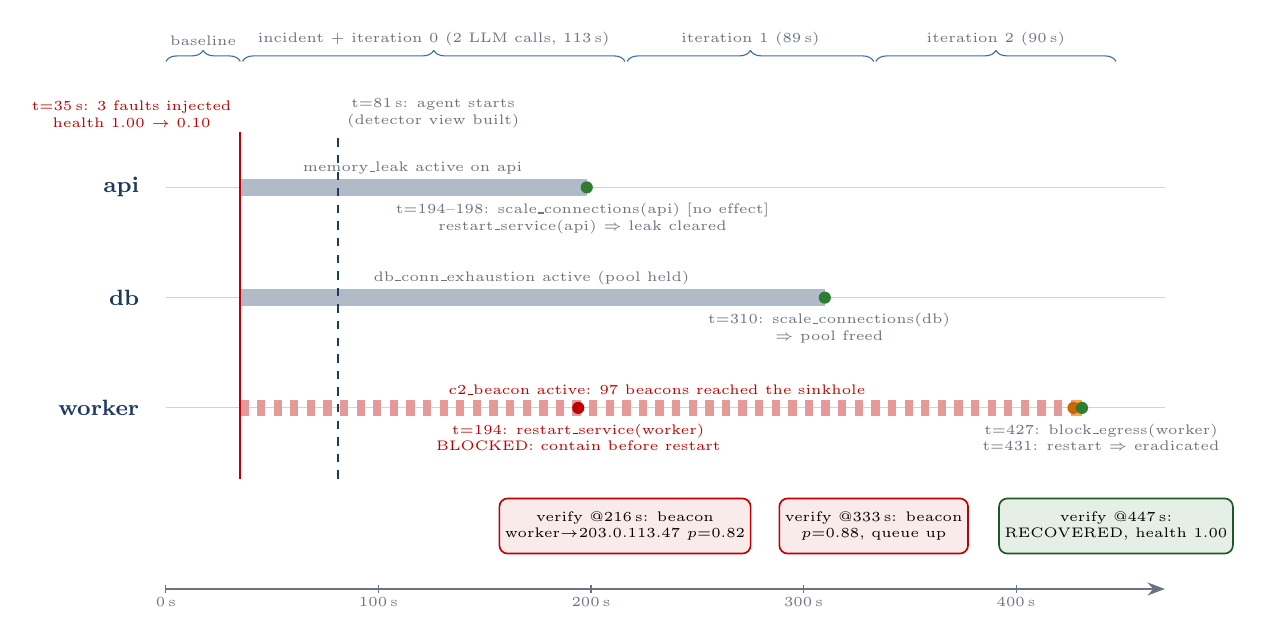
\begin{tikzpicture}[x=0.027cm,y=1cm]
  % lanes
  \foreach \y/\n in {3.4/api,2.0/db,0.6/worker} {
    \node[anchor=east,font=\footnotesize\bfseries,text=accent] at (-8,\y) {\n};
    \draw[gray!35] (0,\y) -- (470,\y);
  }
  % fault bars
  \draw[line width=6pt,accent!35] (35,3.4) -- (198,3.4);
  \node[lbl,above=3pt] at (116,3.4) {memory\_leak active on api};
  \draw[line width=6pt,accent!35] (35,2.0) -- (310,2.0);
  \node[lbl,above=3pt] at (172,2.0) {db\_conn\_exhaustion active (pool held)};
  \draw[line width=6pt,attack!40,dashed] (35,0.6) -- (427,0.6);
  \node[lbl,above=3pt,text=attack] at (231,0.6) {c2\_beacon active: 97 beacons reached the sinkhole};
  \draw[line width=6pt,orange!70] (427,0.6) -- (431,0.6);
  % injection and agent start
  \draw[attack,line width=0.8pt] (35,-0.3) -- (35,4.1);
  \node[lbl,text=attack,anchor=south east] at (33,4.1) {t=35\,s: 3 faults injected\\health 1.00 $\to$ 0.10};
  \draw[accent,line width=0.8pt,dashed] (81,-0.3) -- (81,4.1);
  \node[lbl,anchor=south west] at (83,4.1) {t=81\,s: agent starts\\(detector view built)};
  % actions
  \fill[recovered] (198,3.4) circle (2.2pt);
  \node[lbl,below=4pt] at (196,3.4) {t=194--198: scale\_connections(api) [no effect]\\restart\_service(api) $\Rightarrow$ leak cleared};
  \fill[recovered] (310,2.0) circle (2.2pt);
  \node[lbl,below=4pt] at (312,2.0) {t=310: scale\_connections(db)\\$\Rightarrow$ pool freed};
  \fill[attack] (194,0.6) circle (2.2pt);
  \node[lbl,below=4pt,text=attack] at (194,0.6) {t=194: restart\_service(worker)\\BLOCKED: contain before restart};
  \fill[orange!80!black] (427,0.6) circle (2.2pt);
  \fill[recovered] (431,0.6) circle (2.2pt);
  \node[lbl,below=4pt] at (440,0.6) {t=427: block\_egress(worker)\\t=431: restart $\Rightarrow$ eradicated};
  % verification marks
  \node[bad,font=\tiny,inner sep=2pt] at (216,-0.9) {verify @216\,s: beacon\\worker$\to$203.0.113.47 $p$=0.82};
  \node[bad,font=\tiny,inner sep=2pt] at (333,-0.9) {verify @333\,s: beacon\\$p$=0.88, queue up};
  \node[good,font=\tiny,inner sep=2pt] at (447,-0.9) {verify @447\,s:\\RECOVERED, health 1.00};
  % axis
  \draw[flow,draw=muted] (0,-1.7) -- (470,-1.7);
  \foreach \t in {0,100,200,300,400} { \draw[muted] (\t,-1.75) -- (\t,-1.65); \node[lbl,below] at (\t,-1.75) {\t\,s}; }
  % braces for phases
  \draw[brace] (0,5.0) -- (35,5.0) node[lbl,midway,above=4pt] {baseline};
  \draw[brace] (36,5.0) -- (216,5.0) node[lbl,midway,above=4pt] {incident $+$ iteration 0 (2 LLM calls, 113\,s)};
  \draw[brace] (217,5.0) -- (333,5.0) node[lbl,midway,above=4pt] {iteration 1 (89\,s)};
  \draw[brace] (334,5.0) -- (447,5.0) node[lbl,midway,above=4pt] {iteration 2 (90\,s)};
\end{tikzpicture}}
\caption{The recorded live-demo incident: memory leak on \code{api}, pool exhaustion on \code{db}
and a C2 beacon on \code{worker}, on five real processes. Bars are the hidden fault lifetimes; dots
are the actions that ended them; boxes below the axis are the verifier's verdicts. Times are seconds
since the services started (\code{results/demo\_live\_trace.json}).}
\label{fig:timeline}
\end{figure}

% =====================================================================
\section{Scorer Audit}
\label{sec:audit}
% =====================================================================

Half-way through development, after agent version v2, the recovery metric was challenged with a
concrete suspicion: a dev scenario (\code{dev\_1f\_01}, pool exhaustion on \code{db}) had been scored
as recovered although the agent's first plan was \code{block\_egress(worker)},
\code{restart\_service(worker)}, \code{rollback\_config(api)}. The audit asked five questions and
answered each from saved traces, re-scoring wherever possible instead of re-running.

\paragraph{Why did that run pass?} Because recovery is scored on the \emph{final} ground-truth
state: verification rejected the state after iterations 0 and 1 (``too many connections''), the
model re-planned, and iteration 2 applied \code{scale\_connections(db)}, which resolved the fault.
The leniency was elsewhere: 7 of the 8 actions did nothing, and \code{block\_egress(worker)} on an
uncompromised host was not counted as harmful.

\paragraph{Do faults clear on their own, or via the wrong target?} No. New tests exercise every
fault type through 300 ticks of inaction and through every allow-listed action on every other
service and every wrong action on the right service ($8\times5\times10$). The only cross-service
effect is dependency propagation, which never resolves anything. One real leniency surfaced: with
$H=\overline{h}$, four fault types (latency injection, bad config, beacon, credential stuffing) left
observable health $\ge0.9$ while active, so naive baselines could \emph{claim} recovery.

\paragraph{Sanity floors (dev, 3 seeds, $n=90$ each).} do\_nothing recovers \pct{0} and claims
\pct{3}; random recovers \pct{1}, claims \pct{7} and commits 3.58 harmful actions per run; the
runbook recovers \pct{60}. The recovery check is not broken; both floors stay in the benchmark.

\paragraph{What changed.}
\begin{itemize}
  \item Health became $\tfrac12\overline{h}+\tfrac12\min h$ (\cref{eq:health}); credential stuffing now saturates the auth backend.
  \item \code{action\_precision} and effective-action tracking were added; \code{unnecessary} became applied minus effective (repeated correct actions count).
  \item Containment of a host with no C2 compromise counts as harmful; blocking \code{api}'s egress costs 0.3 error rate while blocked; a restart after containment rebuilds the host and lifts the block.
  \item Rolled-back actions are counted separately but still count as applied.
\end{itemize}

\paragraph{Corrected numbers.} \Cref{tab:audit} shows the dev iteration history re-scored from saved
traces. The pre-audit tables (kept in \code{docs/RESULTS.md} labelled ``pre-audit'') reported
0.00 harmful actions for v0 and v1; the audited scorer shows they blocked egress on uncompromised
hosts 0.27 and 0.23 times per run. The containment gate introduced in v2 (beacon evidence required)
removed that. v3, a full re-run on the audited simulator and scorer, also fixed v2's two false
claims (a known beacon pair had slipped under the strict short-window threshold) and was frozen.

\begin{table}[H]
\centering\small
\caption{Dev-split iteration history, re-scored with the audited scorer (1 seed, $n=30$; runbook 3 seeds, $n=90$). Pre-audit harmful values for v0/v1 were 0.00.}
\label{tab:audit}
\adjustbox{max width=\textwidth}{%
\begin{tabular}{p{6.2cm} r r r r r r r}
\toprule
version & top-1 & recall & recovered & false ``rec.'' & harmful/run & action prec. & calls \\
\midrule
runbook (P2, 3 seeds) & \pct{84} & \pct{84} & \pct{60} & \pct{0} & 0.03 & \pct{72} & 0 \\
agent v0 (first full run) & \pct{70} & \pct{67} & \pct{73} & \pct{0} & \textcolor{attack}{0.27} & \pct{52} & 7.4 \\
agent v1: per-service evidence, down-service rule, repeated-plan guard & \pct{90} & \pct{78} & \pct{100} & \pct{0} & \textcolor{attack}{0.23} & \pct{70} & 4.0 \\
agent v2: containment gate, strict verify, log attribution & \pct{93} & \pct{84} & \pct{93} & \textcolor{attack}{\pct{7}} & 0.00 & \pct{80} & 3.7 \\
\rowcolor{groupfill}agent v3: known-beacon verification \textemdash\ \textbf{frozen} & \pct{90} & \pct{84} & \pct{100} & \pct{0} & 0.00 & \pct{77} & 4.0 \\
\bottomrule
\end{tabular}}
\end{table}

\begin{designdecision}{stop tuning on dev at v3}
v3's remaining top-1 misses are type confusions where the fix coincides (cache latency injection
labelled \code{cache\_failure}, resolved by a restart). Further prompt tuning on those would be
fitting the taxonomy wording to dev, so the agent was frozen (\code{v1-frozen}) and never touched
after the first held-out run.
\end{designdecision}

% =====================================================================
\section{Discussion}
\label{sec:discussion}
% =====================================================================

\paragraph{Division of labour.} The results support a specific claim about where each guarantee
lives. \emph{Diagnosis} comes mostly from the detectors: the runbook, which uses the same thresholds
with no model, reaches top-1 \pct{87}, and removing the beacon detector costs the agent only 7 points
of top-1. \emph{Recovery} comes from the loop: one iteration recovers \pct{20}, the loop \pct{100}.
\emph{Honesty} comes from the verification gate: the same actions produce \pct{0} or \pct{80} false
claims depending only on whether the gate exists. \emph{Harmlessness} comes from the safety layer:
removing it changes recovery by nothing and harm from 0.00 to 0.60 per run. The LLM's contribution
is integration and planning over evidence it did not have to find; when it is given raw telemetry
instead (\code{llm\_only}) its diagnosis collapses to \pct{35} top-1 at six times the cost.

\paragraph{Why the small-model result matters.} \code{qwen2.5:1.5b} recovers only half of the
held-out incidents, loops nearly to the budget (6.0 iterations) and burns almost as many tokens as
\code{llm\_only}. But it makes zero false claims and zero harmful actions. Those two properties are
exactly the ones an operator cannot afford to lose when they downgrade a model for cost, latency or
privacy reasons, and the architecture keeps them independent of model quality: a weaker planner
degrades into an honest escalator, not into a confident liar or a host-restarting hazard.

\paragraph{What the runbook teaches.} A rule-based runbook is a strong diagnoser here because the
symptom vocabulary is fixed, and it is a weak recoverer because it has no notion of cause versus
symptom and no eradication step for a contained implant. Its \pct{5} false claims come from the
\pct{45} of runs where health crossed 0.9 with a fault still active, which the audited health formula
reduced but could not eliminate without ground truth. The gap between \pct{87} top-1 and \pct{45}
recovery is the argument for closing the loop.

\paragraph{Relation to prior benchmarks.} Absolute numbers here are not comparable with ITBench or
OpenRCA: the simulator is small and its symptom signatures are consistent with the taxonomy in the
prompt. What transfers is the evaluation design: multi-fault scenarios with disjoint held-out
combinations, false recovery as a headline metric, security faults inside operational incidents,
cost per incident, sanity floors, and a replay cache that turns every number into a reproducible artefact.

% =====================================================================
\section{Limitations and Threats to Validity}
\label{sec:limits}
% =====================================================================

\begin{limitation}{benchmark realism}
The simulator is small and hand-written: five services, one dependency graph, nine known fault types
with scripted symptom signatures that are consistent with the taxonomy the agent is told, and the
prompt's ``Fix:'' line for each type is generated from that fault class's own accepted remedies
(\code{correct\_sequences()}), the same symptom-to-fix knowledge the runbook baseline hard-codes.
The held-out split tests unseen \emph{combinations} and one unseen \emph{type}, not unseen symptom
vocabularies, so the benchmark measures diagnosis under concurrent faults, safe ordering and
verified recovery more than open-world discovery. Top-1 counts a hit on any injected fault and so
gets easier as faults stack; per-fault recall is the stricter number. Timing is compressed (10\,s ticks, beacons every 25--60\,s); the beacon features are
scale-invariant by construction and by test, but this was demonstrated only between 1.5\,s (live)
and 60\,s (simulator).
\end{limitation}

\begin{limitation}{detector training data and the model}
The beacon RandomForest was trained and tested on synthetic flow timings plus the simulator's dev
scenarios; no real captures were used, and a real deployment would face evasion (very long intervals,
traffic blending) and need retraining on NetFlow or Zeek data. The allow-list is a prior that raises
the bar for trusted destinations rather than a bypass, but a beacon fronted through a trusted CDN
gets that higher bar. \code{qwen2.5:7b} mis-attributes facts between services and ignores status
fields unless they are spelled out; the per-service evidence grouping and the repeated-plan guard
exist because of that.
\end{limitation}

\begin{limitation}{seeds and statistical power}
Agent, runbook, single\_shot, do\_nothing and random use 3 seed offsets per held-out scenario
($n=60$). \code{llm\_only}, the four perturbations, the four ablations and the small-model run use 1
seed ($n=20$; 8 for the unseen fault): their CIs are wide and their deltas should be read as
directional. The 3-seed \code{llm\_only} pass was started twice and stopped at 10/60 both times
because raw-telemetry prompts make it about five times slower; both attempts are in
\code{results/heldout\_runs.log}. The brief asked for benchmark commands under 15 minutes; with a 7B
model on a fanless laptop the held-out commands take 29--95 minutes and fewer seeds were chosen over
fewer scenarios. \code{make smoke} and CI run from the cache in under a minute.
\end{limitation}

\begin{limitation}{replay is exact, re-recording is not}
Every reported number replays bit-for-bit from the committed cache, and CI checks it on every
push (\code{bench/replay\_check.py}). That check found one bug: the timestamp-jitter wrapper salted
its noise with Python's per-process string \code{hash()}, so that split could not be replayed; it
now uses a stable CRC32 salt and the split was re-recorded with identical headline numbers. Re-running against Ollama can
produce slightly different completions even at temperature 0 (batched decoding is not bit-stable),
so a fresh recording is a new experiment, not a reproduction. The live environment is a demo and a
``same agent, two environments'' test, not a second benchmark: its timing is non-deterministic and
the cache does not apply.
\end{limitation}

\begin{limitation}{safety layer and scope}
Rollback is best-effort: restarts, config rollbacks, disk clears and cache flushes are irreversible
and recorded as such. The evidence gate trusts the detector's beacon findings; with the detector off
it trusts the model's hypothesis list, so a wrong \code{c2\_beacon} hypothesis on an innocent host
would unlock its containment (the regression check catches the availability loss on hosts with
external dependencies, not a silent block on a host that needs no egress). Isolation and egress
blocking in the live environment are flags inside the process, not real network policy. There is no
multi-cluster topology, no autoscaling, no network partition and no multi-step attack (lateral
movement, exfiltration); a fault whose fix is outside the eight-action allowlist is unrecoverable by
design and escalates.
\end{limitation}

% =====================================================================
\section{Path to Production}
\label{sec:production}
% =====================================================================

The architecture was chosen so that each component has an obvious production counterpart.
\begin{enumerate}
  \item \textbf{Telemetry adapters.} Replace the simulator's flow records with NetFlow/Zeek
        connection logs and the metric and log readers with Prometheus and a log store behind the same
        \code{Env} interface; the detectors and the agent do not change.
  \item \textbf{Beacon model.} Retrain the RandomForest on real captures (the feature set is the one
        validated on CTU-13 in prior work~\cite{alharbi-thesis}); keep destination knowledge as a prior,
        and add long-interval windows.
  \item \textbf{Actions.} Map the eight allow-listed actions to existing runbook automations behind
        the same safety layer; require human approval for irreversible actions (restart, rollback,
        clear, flush) and keep containment automatic but evidence-gated.
  \item \textbf{Verification as the only path to ``resolved''.} Keep the gate, the remembered healthy
        baseline and the known-pair rule; make the verifier's problem list the incident's status
        page.
  \item \textbf{Model.} The loop needs a JSON-mode model with a few thousand tokens of context; a
        privately hosted model is sufficient, and the record/replay cache doubles as an audit log of
        every decision the model made.
  \item \textbf{Regression discipline.} Keep the smoke subset and the sanity floors in CI; add every
        real incident as a replayable scenario.
\end{enumerate}

% =====================================================================
\section{Conclusion}
% =====================================================================

Sentinel-RX treats a failing enterprise system as a security problem as much as an operations
problem, and treats the agent's own claims as something to be verified rather than believed. On
twenty held-out incidents with up to three concurrent faults and hidden C2 beacons, a local 7B model
wrapped in deterministic detectors, a safety layer and a verification gate recovered every system,
never claimed a recovery it had not achieved, and never restarted a compromised host before
containing it, at about six thousand tokens per incident. Ablations locate each of those properties in
a specific component, perturbations show they survive degraded telemetry and degrade safely on an unseen fault type,
and a smaller model shows that honesty and harmlessness do not depend on model quality. The scorer
that produced these numbers was audited mid-way, found lenient in two places, fixed and re-applied
to every earlier run. Everything, from the simulator to the replay cache that reproduces the tables
without a model, runs on one laptop and is included.

% =====================================================================
\begin{thebibliography}{99}
\small
\bibitem{kephart} J.~O. Kephart and D.~M. Chess, ``The vision of autonomic computing,'' \emph{IEEE Computer}, vol.~36, no.~1, pp.~41--50, 2003.
\bibitem{chaos} A.~Basiri, N.~Behnam, R.~de~Rooij, L.~Hochstein, L.~Kosewski, J.~Reynolds, and C.~Rosenthal, ``Chaos engineering,'' \emph{IEEE Software}, vol.~33, no.~3, pp.~35--41, 2016.
\bibitem{notaro} P.~Notaro, J.~Cardoso, and M.~Gerndt, ``A survey of AIOps methods for failure management,'' \emph{ACM Trans. Intelligent Systems and Technology}, vol.~12, no.~6, art.~81, 2021.
\bibitem{rcacopilot} Y.~Chen, H.~Xie, M.~Ma, Y.~Kang, X.~Gao, L.~Shi, Y.~Cao, X.~Gao, H.~Fan, M.~Wen, J.~Zeng, S.~Ghosh, X.~Zhang, C.~Zhang, Q.~Lin, S.~Rajmohan, D.~Zhang, and T.~Xu, ``Automatic root cause analysis via large language models for cloud incidents,'' in \emph{Proc. 19th European Conf. on Computer Systems (EuroSys)}, 2024.
\bibitem{rcagent} Z.~Wang, Z.~Liu, Y.~Zhang, A.~Zhong, J.~Wang, F.~Yin, L.~Fan, L.~Wu, and Q.~Wen, ``RCAgent: Cloud root cause analysis by autonomous agents with tool-augmented large language models,'' in \emph{Proc. 33rd ACM Int. Conf. on Information and Knowledge Management (CIKM)}, 2024.
\bibitem{react} S.~Yao, J.~Zhao, D.~Yu, N.~Du, I.~Shafran, K.~Narasimhan, and Y.~Cao, ``ReAct: Synergizing reasoning and acting in language models,'' in \emph{Proc. 11th Int. Conf. on Learning Representations (ICLR)}, 2023.
\bibitem{aiopslab-vision} M.~Shetty, Y.~Chen, G.~Somashekar, M.~Ma, Y.~Simmhan, X.~Zhang, J.~Mace, D.~Vandevoorde, P.~Las-Casas, S.~M. Gupta, S.~Nath, C.~Bansal, and S.~Rajmohan, ``Building AI agents for autonomous clouds: Challenges and design principles,'' in \emph{Proc. ACM Symposium on Cloud Computing (SoCC)}, 2024, pp.~99--110.
\bibitem{aiopslab} Y.~Chen, M.~Shetty, G.~Somashekar, M.~Ma, Y.~Simmhan, J.~Mace, C.~Bansal, R.~Wang, and S.~Rajmohan, ``AIOpsLab: A holistic framework to evaluate AI agents for enabling autonomous clouds,'' in \emph{Proc. 8th Conf. on Machine Learning and Systems (MLSys)}, 2025.
\bibitem{itbench} S.~Jha \emph{et al.}, ``ITBench: Evaluating AI agents across diverse real-world IT automation tasks,'' in \emph{Proc. 42nd Int. Conf. on Machine Learning (ICML)}, PMLR vol.~267, 2025, pp.~27134--27197.
\bibitem{openrca} J.~Xu, Q.~Zhang, Z.~Zhong, S.~He, C.~Zhang, Q.~Lin, D.~Pei, P.~He, D.~Zhang, and Q.~Zhang, ``OpenRCA: Can large language models locate the root cause of software failures?'' in \emph{Proc. 13th Int. Conf. on Learning Representations (ICLR)}, 2025.
\bibitem{rcaeval} L.~Pham, H.~Zhang, H.~Ha, F.~Salim, and X.~Zhang, ``RCAEval: A benchmark for root cause analysis of microservice systems with telemetry data,'' in \emph{Companion Proc. ACM Web Conference (WWW Companion)}, 2025.
\bibitem{stratus} Y.~Chen, J.~Pan, J.~Clark, Y.~Su, N.~Zheutlin, B.~Bhavya, R.~R. Arora, Y.~Deng, S.~Jha, and T.~Xu, ``STRATUS: A multi-agent system for autonomous reliability engineering of modern clouds,'' in \emph{Advances in Neural Information Processing Systems (NeurIPS)}, vol.~38, 2025.
\bibitem{toolemu} Y.~Ruan, H.~Dong, A.~Wang, S.~Pitis, Y.~Zhou, J.~Ba, Y.~Dubois, C.~J. Maddison, and T.~Hashimoto, ``Identifying the risks of LM agents with an LM-emulated sandbox,'' in \emph{Proc. 12th Int. Conf. on Learning Representations (ICLR)}, 2024.
\bibitem{baywatch} X.~Hu, J.~Jang, M.~P. Stoecklin, T.~Wang, D.~L. Schales, D.~Kirat, and J.~R. Rao, ``BAYWATCH: Robust beaconing detection to identify infected hosts in large-scale enterprise networks,'' in \emph{Proc. 46th Annual IEEE/IFIP Int. Conf. on Dependable Systems and Networks (DSN)}, 2016, pp.~479--490.
\bibitem{ctu13} S.~Garc\'ia, M.~Grill, J.~Stiborek, and A.~Zunino, ``An empirical comparison of botnet detection methods,'' \emph{Computers \& Security}, vol.~45, pp.~100--123, 2014.
\bibitem{alharbi-thesis} A.~Alharbi, ``Periodicity-based triage of APT command-and-control beaconing in network flows using machine learning,'' M.S. thesis, Dept. of Computer Science, University of Nevada, Las Vegas, 2026.
\end{thebibliography}

% =====================================================================
\appendix
\section{Reproduction commands}
\label{app:repro}
% =====================================================================
All commands run from the repository root on macOS or Linux with Python~3.12. Replay targets need no
LLM; recording targets need Ollama at \code{localhost:11434} with \code{qwen2.5:7b}
(and \code{qwen2.5:1.5b} for the small-model run).

\begin{tcolorbox}[enhanced,colback=keyfill,colframe=accent!60,boxrule=0.5pt,arc=2pt,left=6pt,right=6pt]
\scriptsize\begin{verbatim}
make setup          # venv, pinned deps, scenarios, beacon detector training (~1 min)
make test           # 109 tests, no LLM needed
make lint           # ruff check + ruff format --check
make smoke          # 5 dev scenarios from the replay cache, no LLM (< 60 s); CI adds floors
make demo-live      # 5 real local processes + 3 concurrent faults + the agent (needs Ollama)
make bench-heldout  # agent, runbook, single_shot, llm_only on held-out, 3 seeds, --final
make bench-perturb  # 5 perturbation sets + the qwen2.5:1.5b run, --final
make ablate         # no_verify, no_loop, no_beacon, no_safety on held-out, --final
make report         # results/summary.md, docs/figures/*.png, site/data.json
make all-final      # test + bench-heldout + bench-perturb + ablate + report (hours)

# exact replay of a reported table from the committed cache, no model needed:
python -m bench.runner --split heldout --config agent --seeds 3 --final --replay
python -m bench.runner --split heldout --config do_nothing,random --seeds 3 --final
python -m bench.rescore results/<run>.json   # re-score saved traces, current scorer
python -m http.server -d site 8000           # leaderboard, charts, replay viewer
\end{verbatim}
\end{tcolorbox}

The held-out run log (\code{results/heldout\_runs.log}) records the UTC time, split, configurations,
model and git revision of every non-dev run, including the two stopped \code{llm\_only} attempts.

% =====================================================================
\clearpage
\section{Repository map}
\label{app:map}
% =====================================================================
\begin{table}[H]
\centering\small
\begin{tabularx}{\textwidth}{l X}
\toprule
path & contents \\
\midrule
\code{env/base.py}, \code{env/types.py} & \code{Env} interface, observable health (\cref{eq:health}), telemetry types, the 8-action allowlist \\
\code{env/sim/} & deterministic simulator: hidden world and propagation (\code{world.py}), telemetry, actions, ground truth (\code{sim\_env.py}) \\
\code{env/live/} & five real local services, in-process fault injection, sinkhole, supervision, \code{make demo-live} \\
\code{env/perturb.py} & observation-layer perturbation wrappers \\
\code{faults/} & 9 known fault types + held-out \code{dns\_failure}; symptoms, correct sequences, harmful-action rules \\
\code{scenarios/} & YAML schema, generator with split guards, committed \code{dev/}, \code{heldout/}, \code{perturbations/} \\
\code{agent/detectors/} & metric z-scores, log templates, dependency ranker, beacon RandomForest and trainer, evidence builder and verifier \\
\code{agent/loop.py}, \code{agent/safety.py} & MAPE-K loop with step budget (\cref{alg:loop}); safety layer (\cref{fig:safety}) \\
\code{agent/llm.py}, \code{agent/prompts.py}, \code{agent/schema.py} & Ollama client with content-addressed record/replay cache; prompts with the fault taxonomy; JSON validation \\
\code{agent/runbook.py}, \code{agent/baselines.py} & runbook, single\_shot, do\_nothing and random baselines \\
\code{bench/} & scorer (all metric definitions), bootstrap aggregation, runner with held-out guard, re-scorer, report, smoke gate \\
\code{models/} & trained beacon RandomForest and its metrics (\cref{fig:pr}) \\
\code{cache/} & committed LLM responses keyed by content hash \\
\code{results/} & result JSON per run, per-scenario traces, \code{summary.md}, \code{heldout\_runs.log}, live-demo console and trace \\
\code{docs/} & \code{DESIGN.md}, \code{RESULTS.md} (dev iteration log and audit), \code{LIMITATIONS.md}, \code{JUDGING.md}, figures, literature review, this report \\
\code{site/} & static leaderboard, charts and incident replay viewer reading \code{site/data.json} \\
\code{tests/} & 109 tests (simulator, faults, scenarios, detectors, agent with scripted LLM, scorer, runner, live environment) \\
\code{.github/workflows/ci.yml} & ruff, pytest, \code{make smoke} from the cache, regression floors \\
\bottomrule
\end{tabularx}
\end{table}

\end{document}
